
%summary of the previous chapters

Usually epicardial leads are labeled \gls{mri}-conditional at best \cite{schaller2021,fda2023testing}. Leaving uncertainties on whether patients with these leads can undergo a \gls{mri} scan, despite the fact that these patient population is more likely to need one. 

The different lead types, uni-polar vs bipolar, materials they are made of, size and configuration, and case by case complications pose a real challenge in the identification and testing of these leads under a \gls{mri} environment. Moreover, the effects on the leads are split by physical interaction. Being three the major concerns RF induced-heating, magnetically induced forces and torques, and electrical currents produced by gradient encoders.

In Chapter \ref{ch:background} an explanation on the physics for the particular case of magnetically induced force and torques is given. Leaning into our methodology which has a three step approach with expected measurement limits. 

For this chapter, we present the results found on each of the experiments parallel to Chapter \ref{ch:matsNmets}, that is Magnetic field mapping, Translational Force Measurements, and Torque measurements. In each of these experiments, the focus is on both laboratory work and clinical work. First, the laboratory work shows the expected behavior in a safe, controllable manner and allows us to predict the results on the clinic. Second, the clinical work will orient us and allow for assumption check and methodology fixes. This changes will be addressed in Chapter \ref{ch:disCon}.

%"The fool collects facts; the wise man selects them" %I am the fool
%past tense
%what you did and what you found
\section{Magnetic Field Mapping}
\subsection{Mapping for a Solenoid in Lab}

The magnetic field $B$ generated in section \ref{sec:FieldGeneration}, yielded to the following figures. In this particular set of measurements the main objective is to capture the spatial gradient behavior of an static magnetic field produced by a solenoid, which has a constant current flow throughout the experiment. Figure \ref{fig:bfield_time_z} shows two plots from the field mapped, Fig. \ref{fig:bfield_time} shows the magnetic field flux B in gauss as a function of time going in and out to the solenoid front face, while Fig. \ref{fig:bfield_z} shows the estimated respective positions of the probe along the z-axis.


\begin{figure}[hbt!]
	\centering
	\subfigure[$B$ field as a function of time.\label{fig:bfield_time}]{
		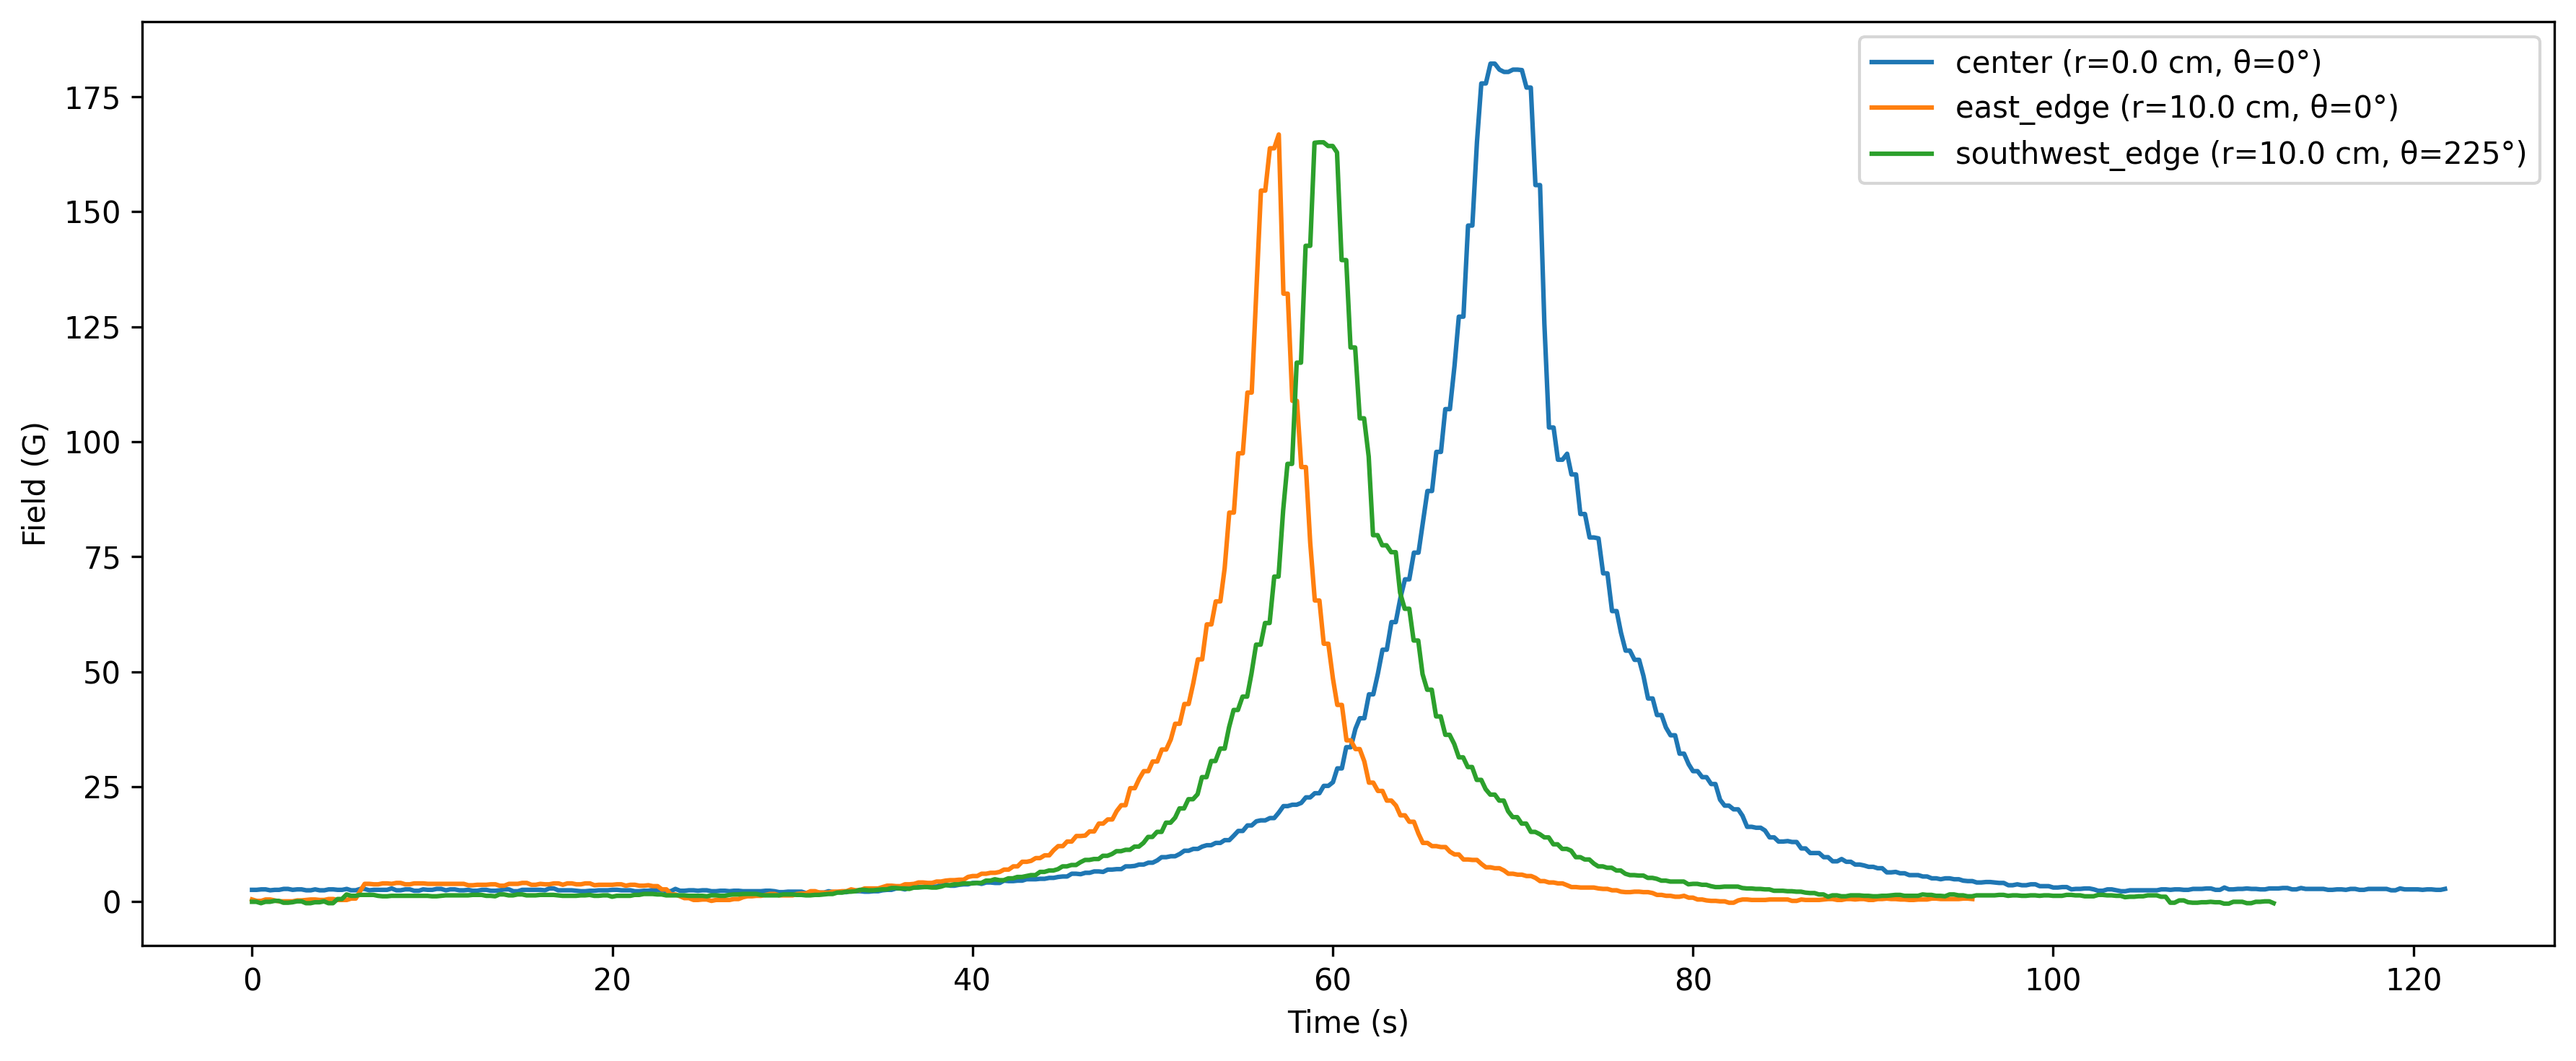
\includegraphics[width=0.9\textwidth]{Assets/BfieldvsTime.png}
	}
	\hfill
	\subfigure[$B$ field as a function of $z$-position.\label{fig:bfield_z}]{
		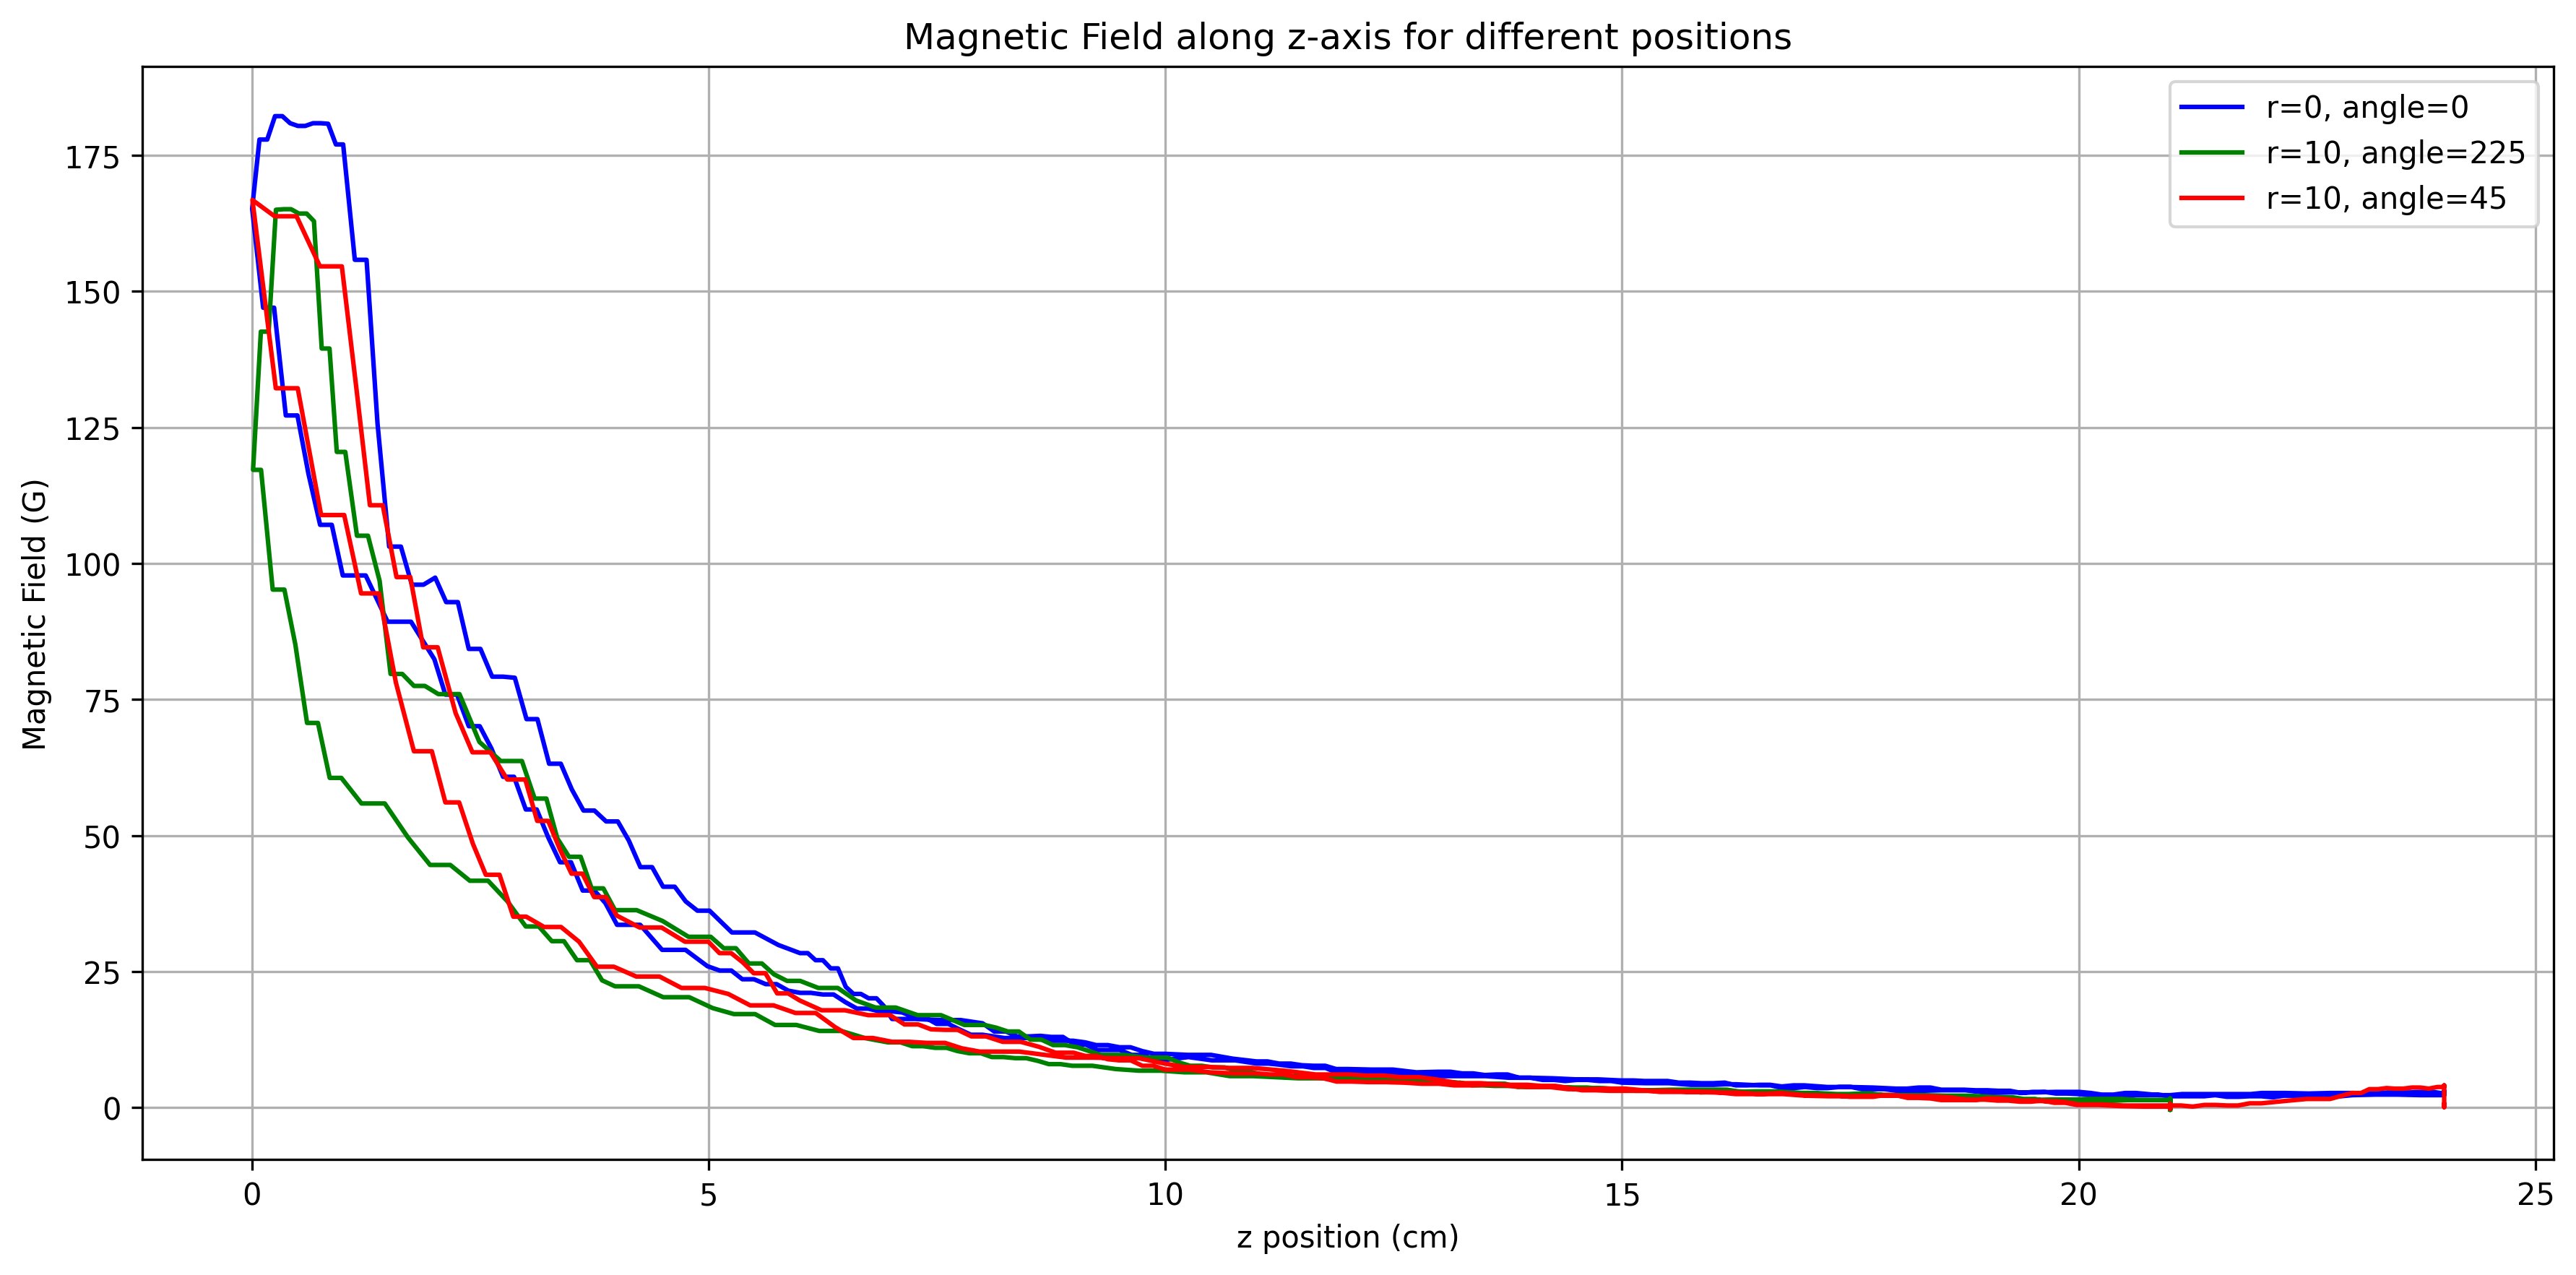
\includegraphics[width=0.8\textwidth]{Assets/BfieldvsZ.png}
	}
	
	\caption[$B$-field behavior along time and displacement]{Magnetic field measurements plotted against time and axial displacement. Used to estimate stability and spatial variation of the mapping setup.}
	\label{fig:bfield_time_z}
\end{figure}

The three colors represent the position of the probe on each trial, this can be seen clearly on Figure \ref{fig:bfield3d} where the map was plotted as a representative line for their respective side. It is important to notice the similarities between runs on the southwest side and the east side of the front as this expected homogeneity allow us to extrapolate the data around the solenoid similar to Fig \ref{fig:3D_field_plot} confirming the theoretical background and speeding our clinical magnetic field acquisition protocol.


\begin{figure}[htb!]
	\centering
	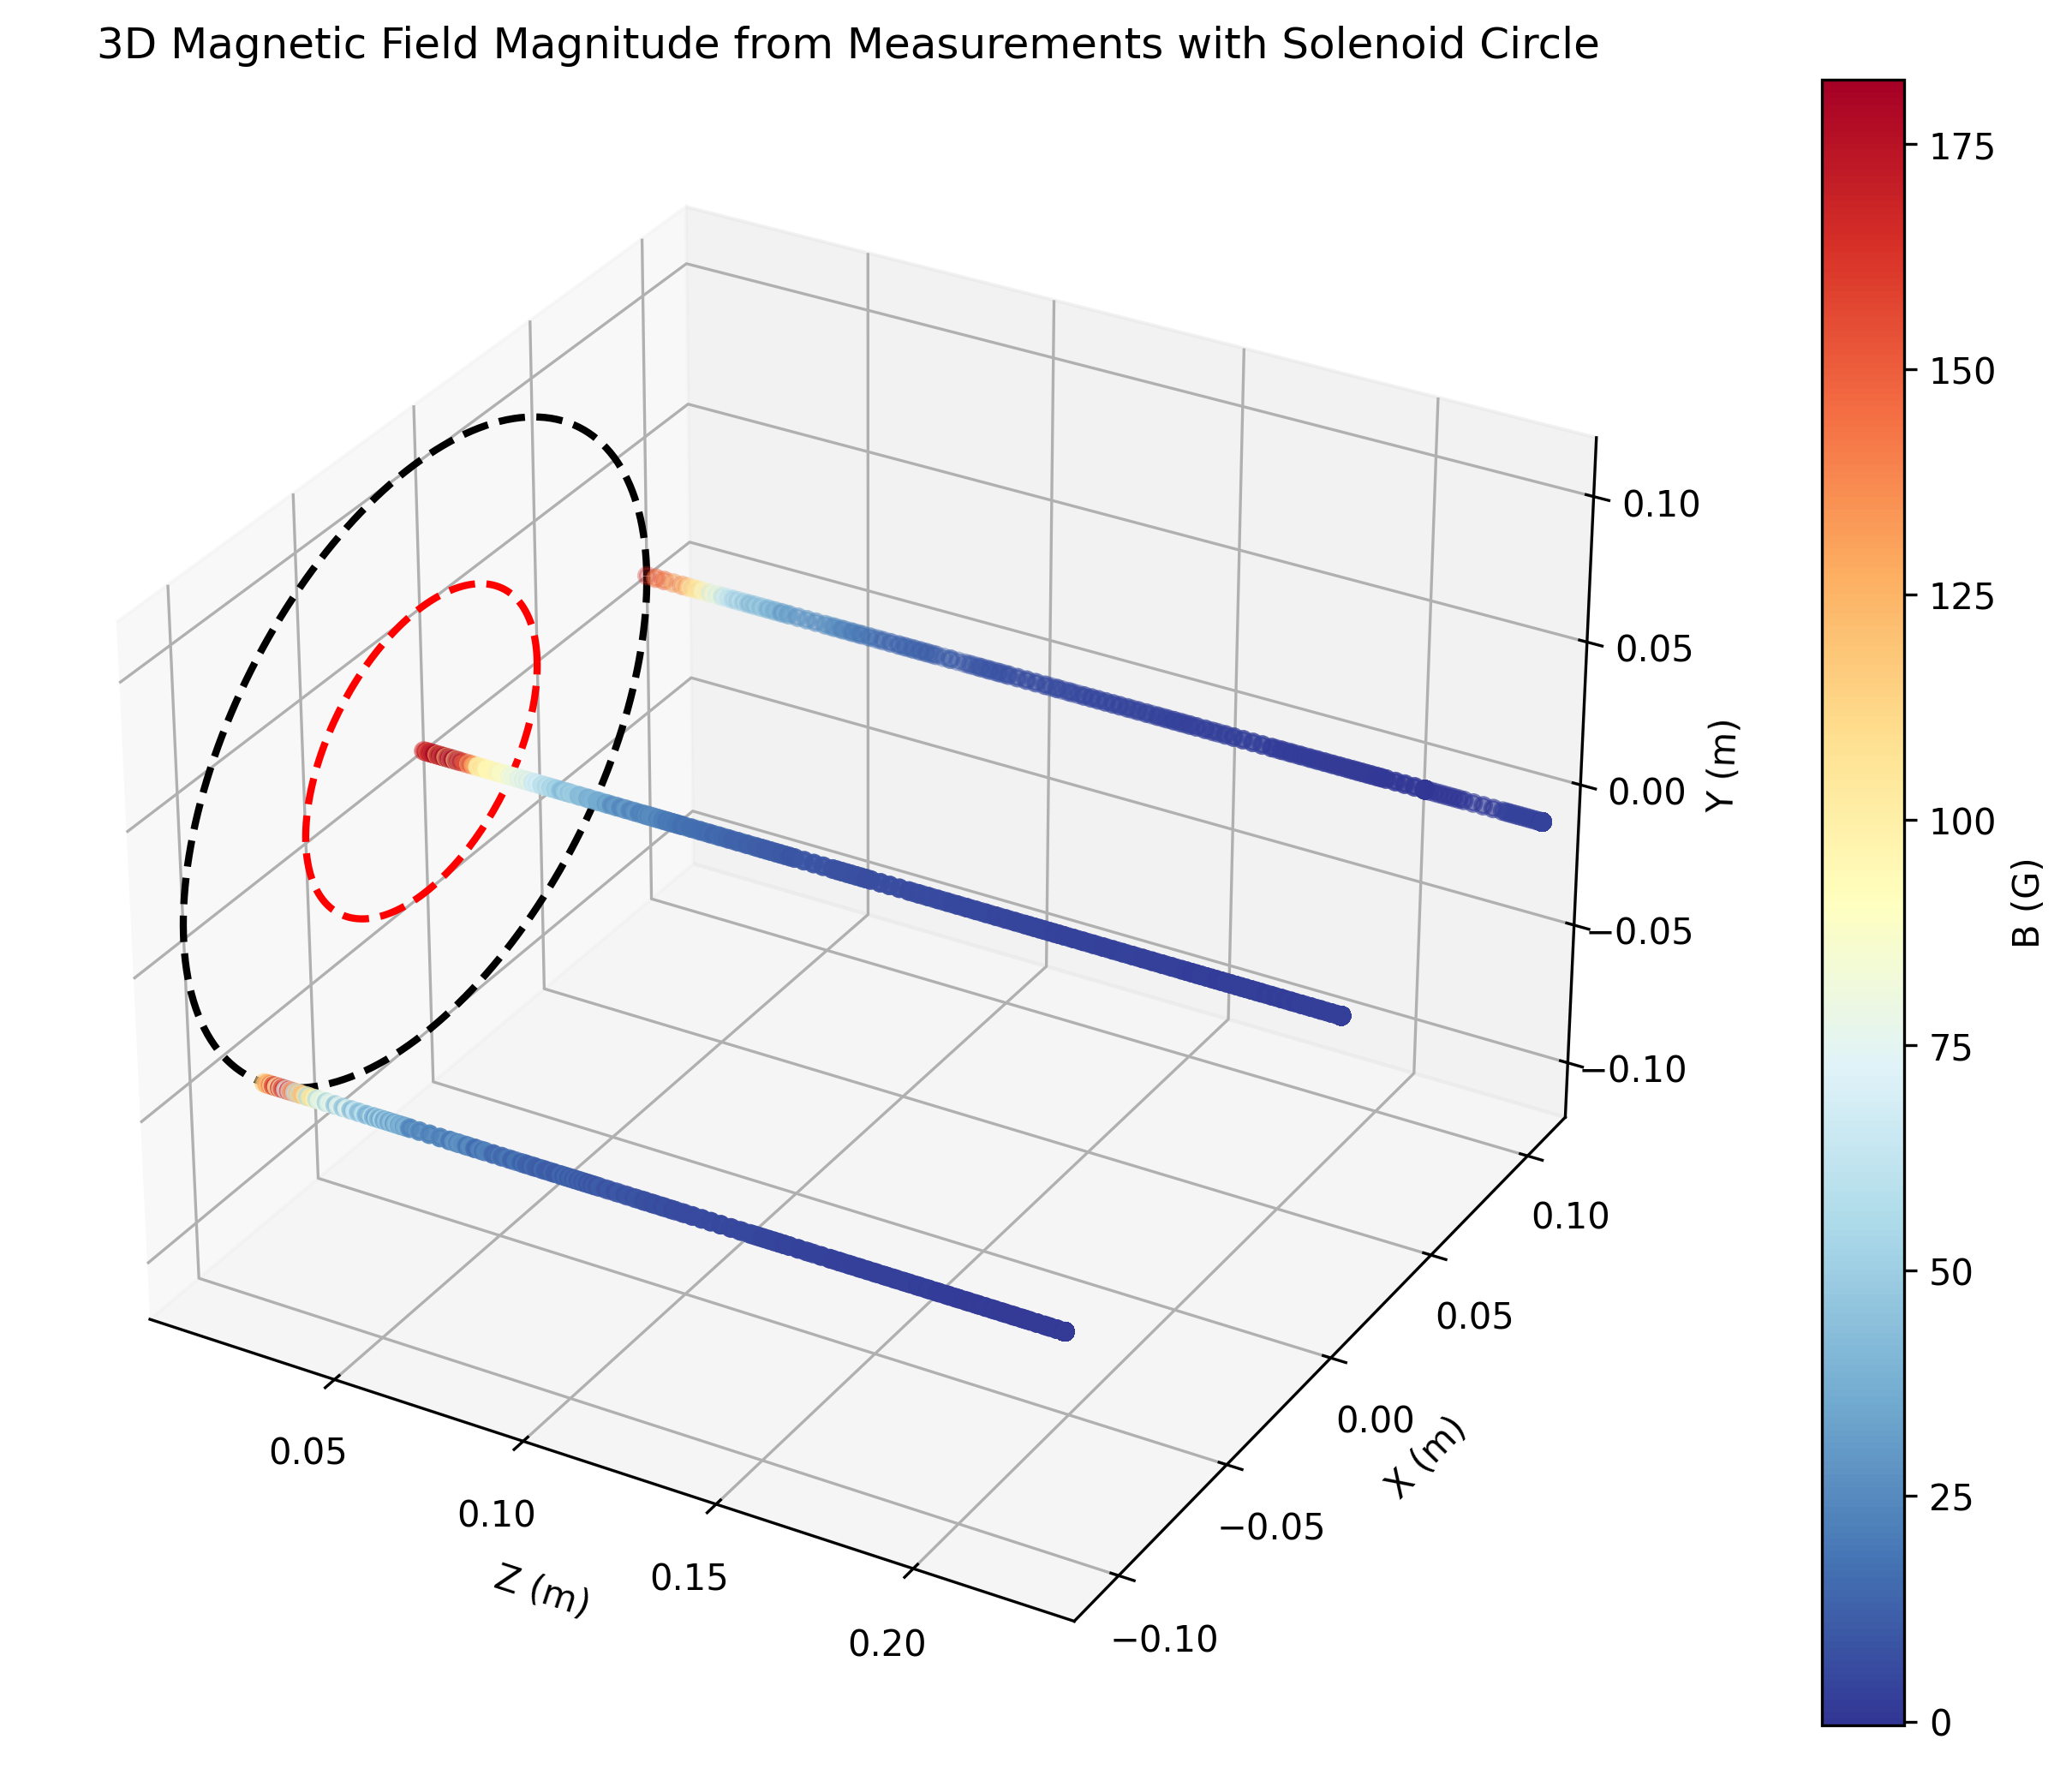
\includegraphics[width=0.75\textwidth]{Assets/Bfield3dreal.png}
	\caption[3D reconstructed field map]{Three-dimensional reconstruction of the measured magnetic field, illustrating spatial variation across the mapping region.}
	\label{fig:bfield3d}
\end{figure}

Figure \ref{fig:gradb_pair} shows both the calculated gradient from equation \ref{eq:finiteDiff}, and the multiplication by field strength $B$ at the particular current of 2.966 A. The later being useful on experiment \ref{sec:Translational} for finding magnetic force, as per equation \ref{eq:translationalForce}, and for its fit (see Eq.\ref{eq:forFit}) making one point out of the set in the translational experiment described in section \ref{sec:experiment1}.

\begin{figure}[hbt!]
	\centering
	\subfigure[$\nabla B$ along the measurement path.\label{fig:gradb}]{
		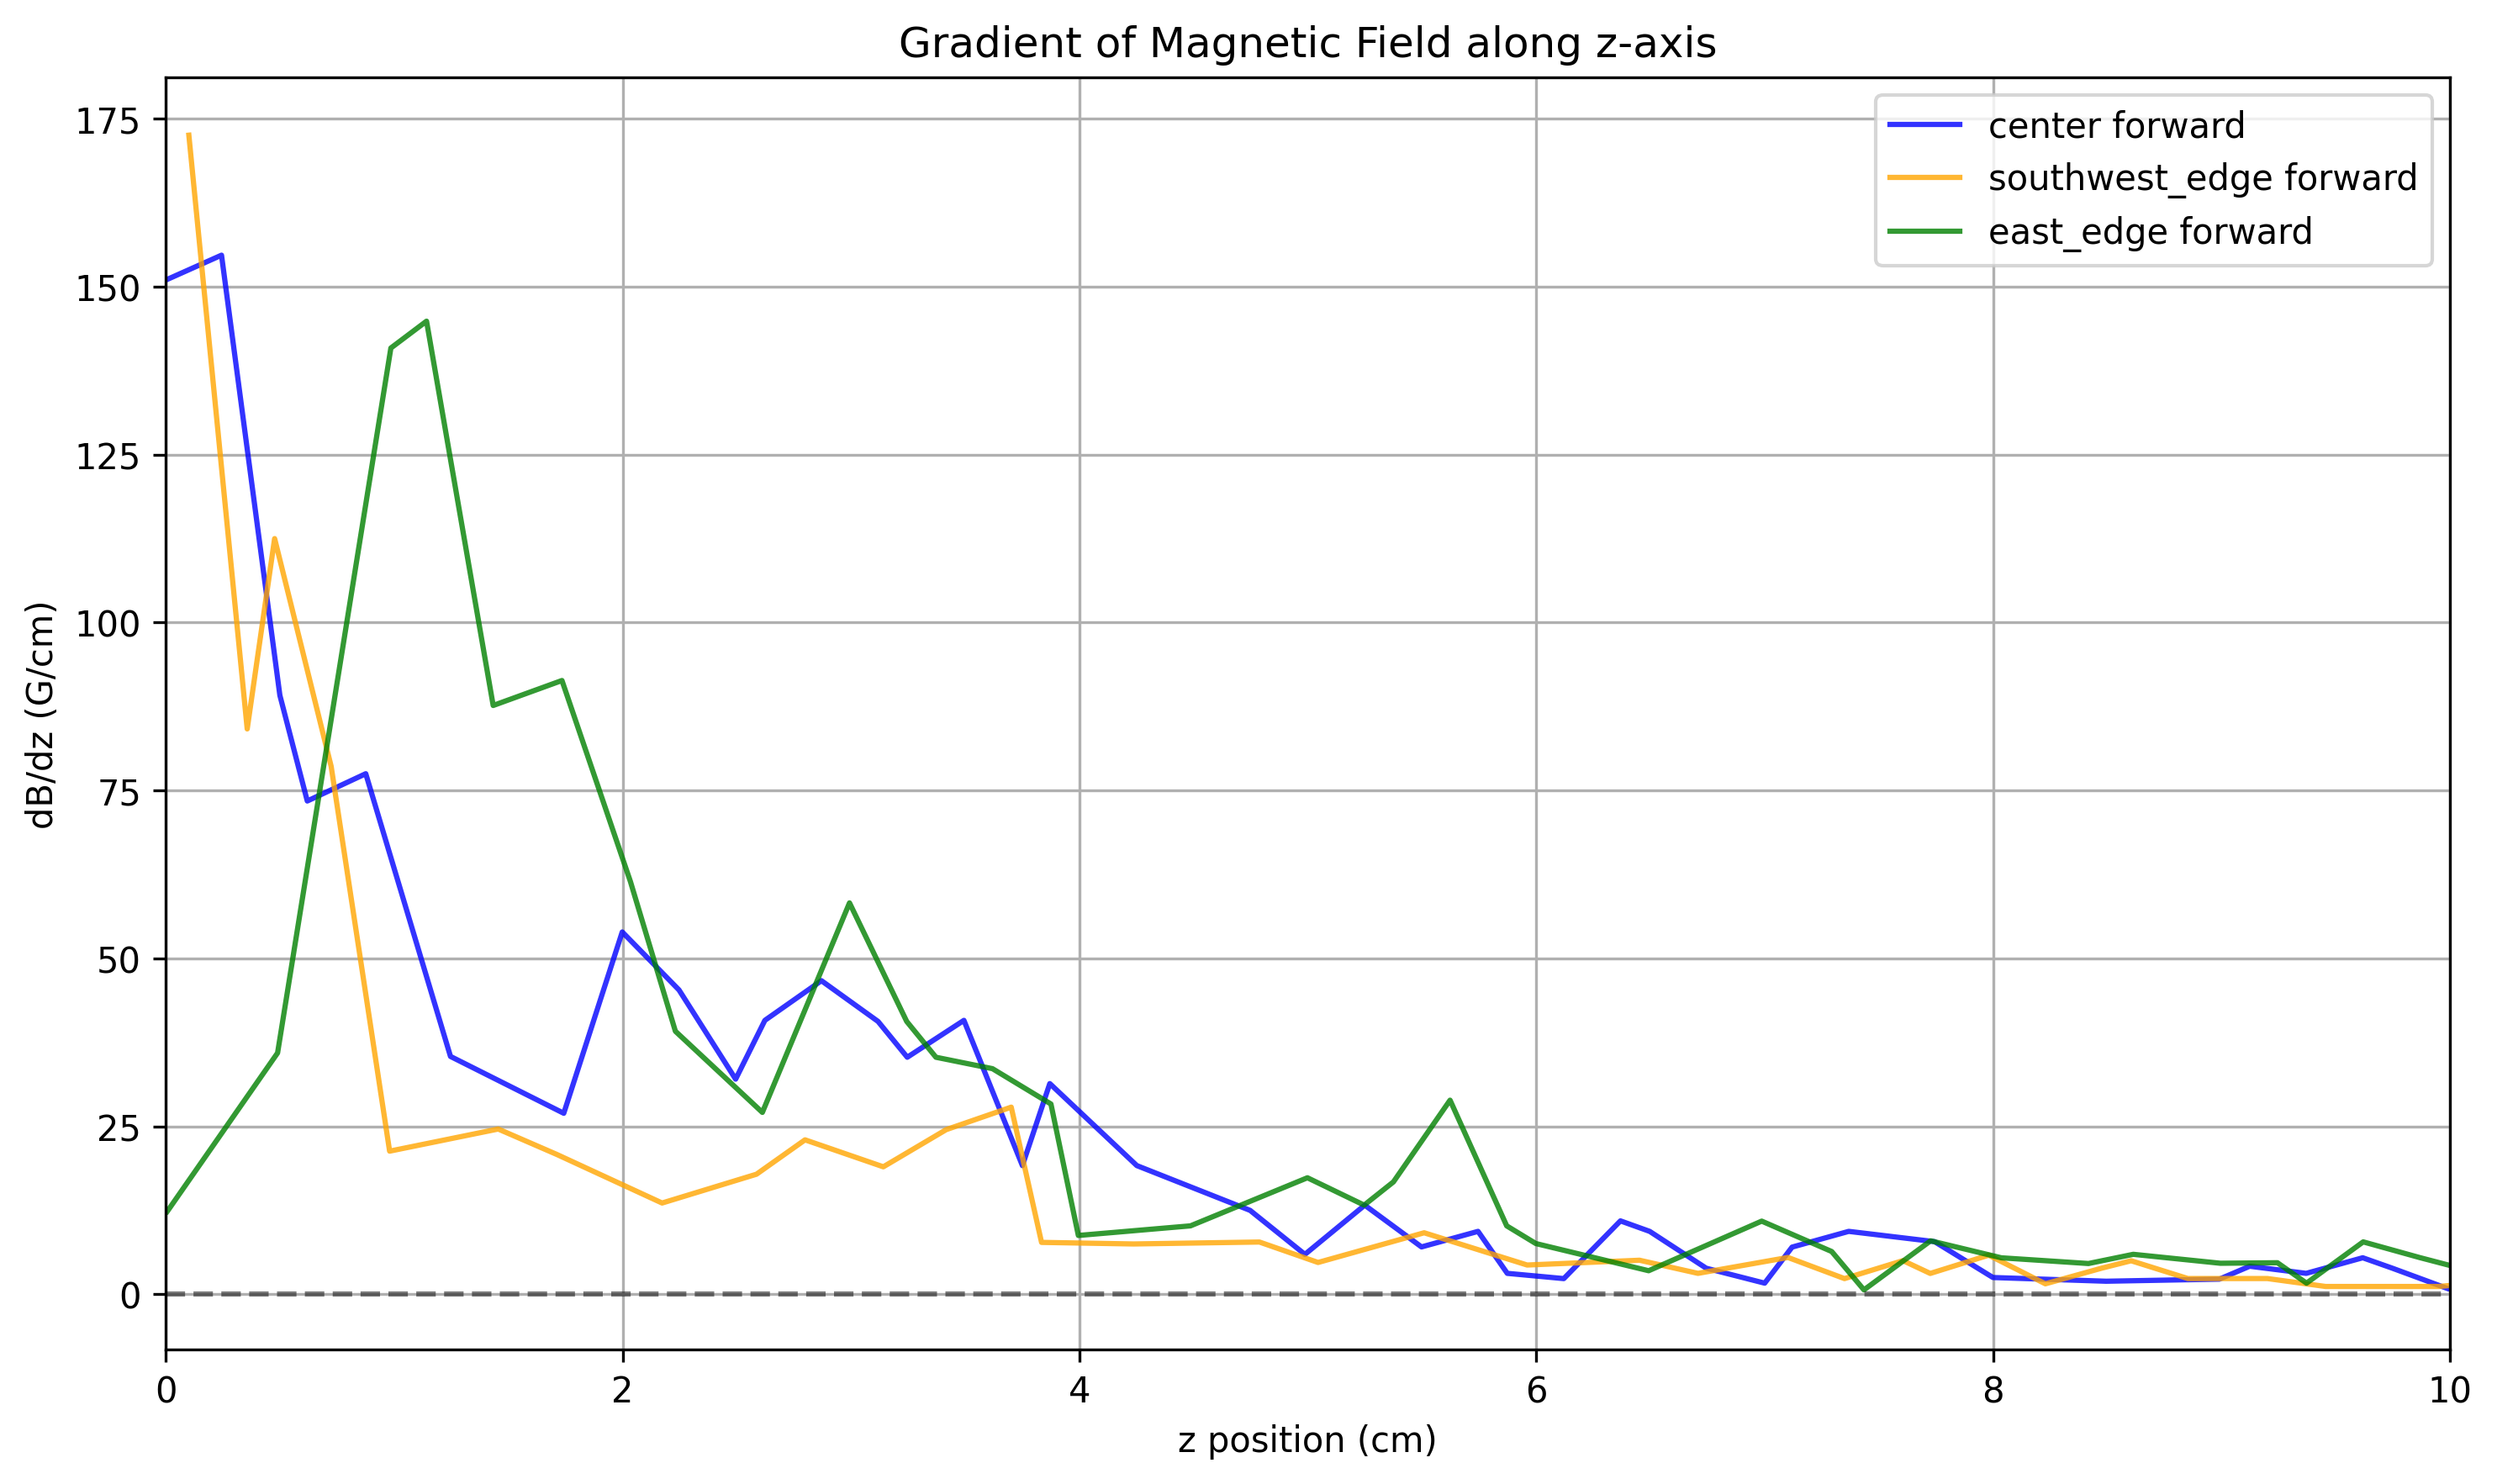
\includegraphics[width=0.90\textwidth]{Assets/gradB.png}
	}
	\hfill
	\subfigure[$B\nabla B$ product along the path.\label{fig:b_gradb}]{
		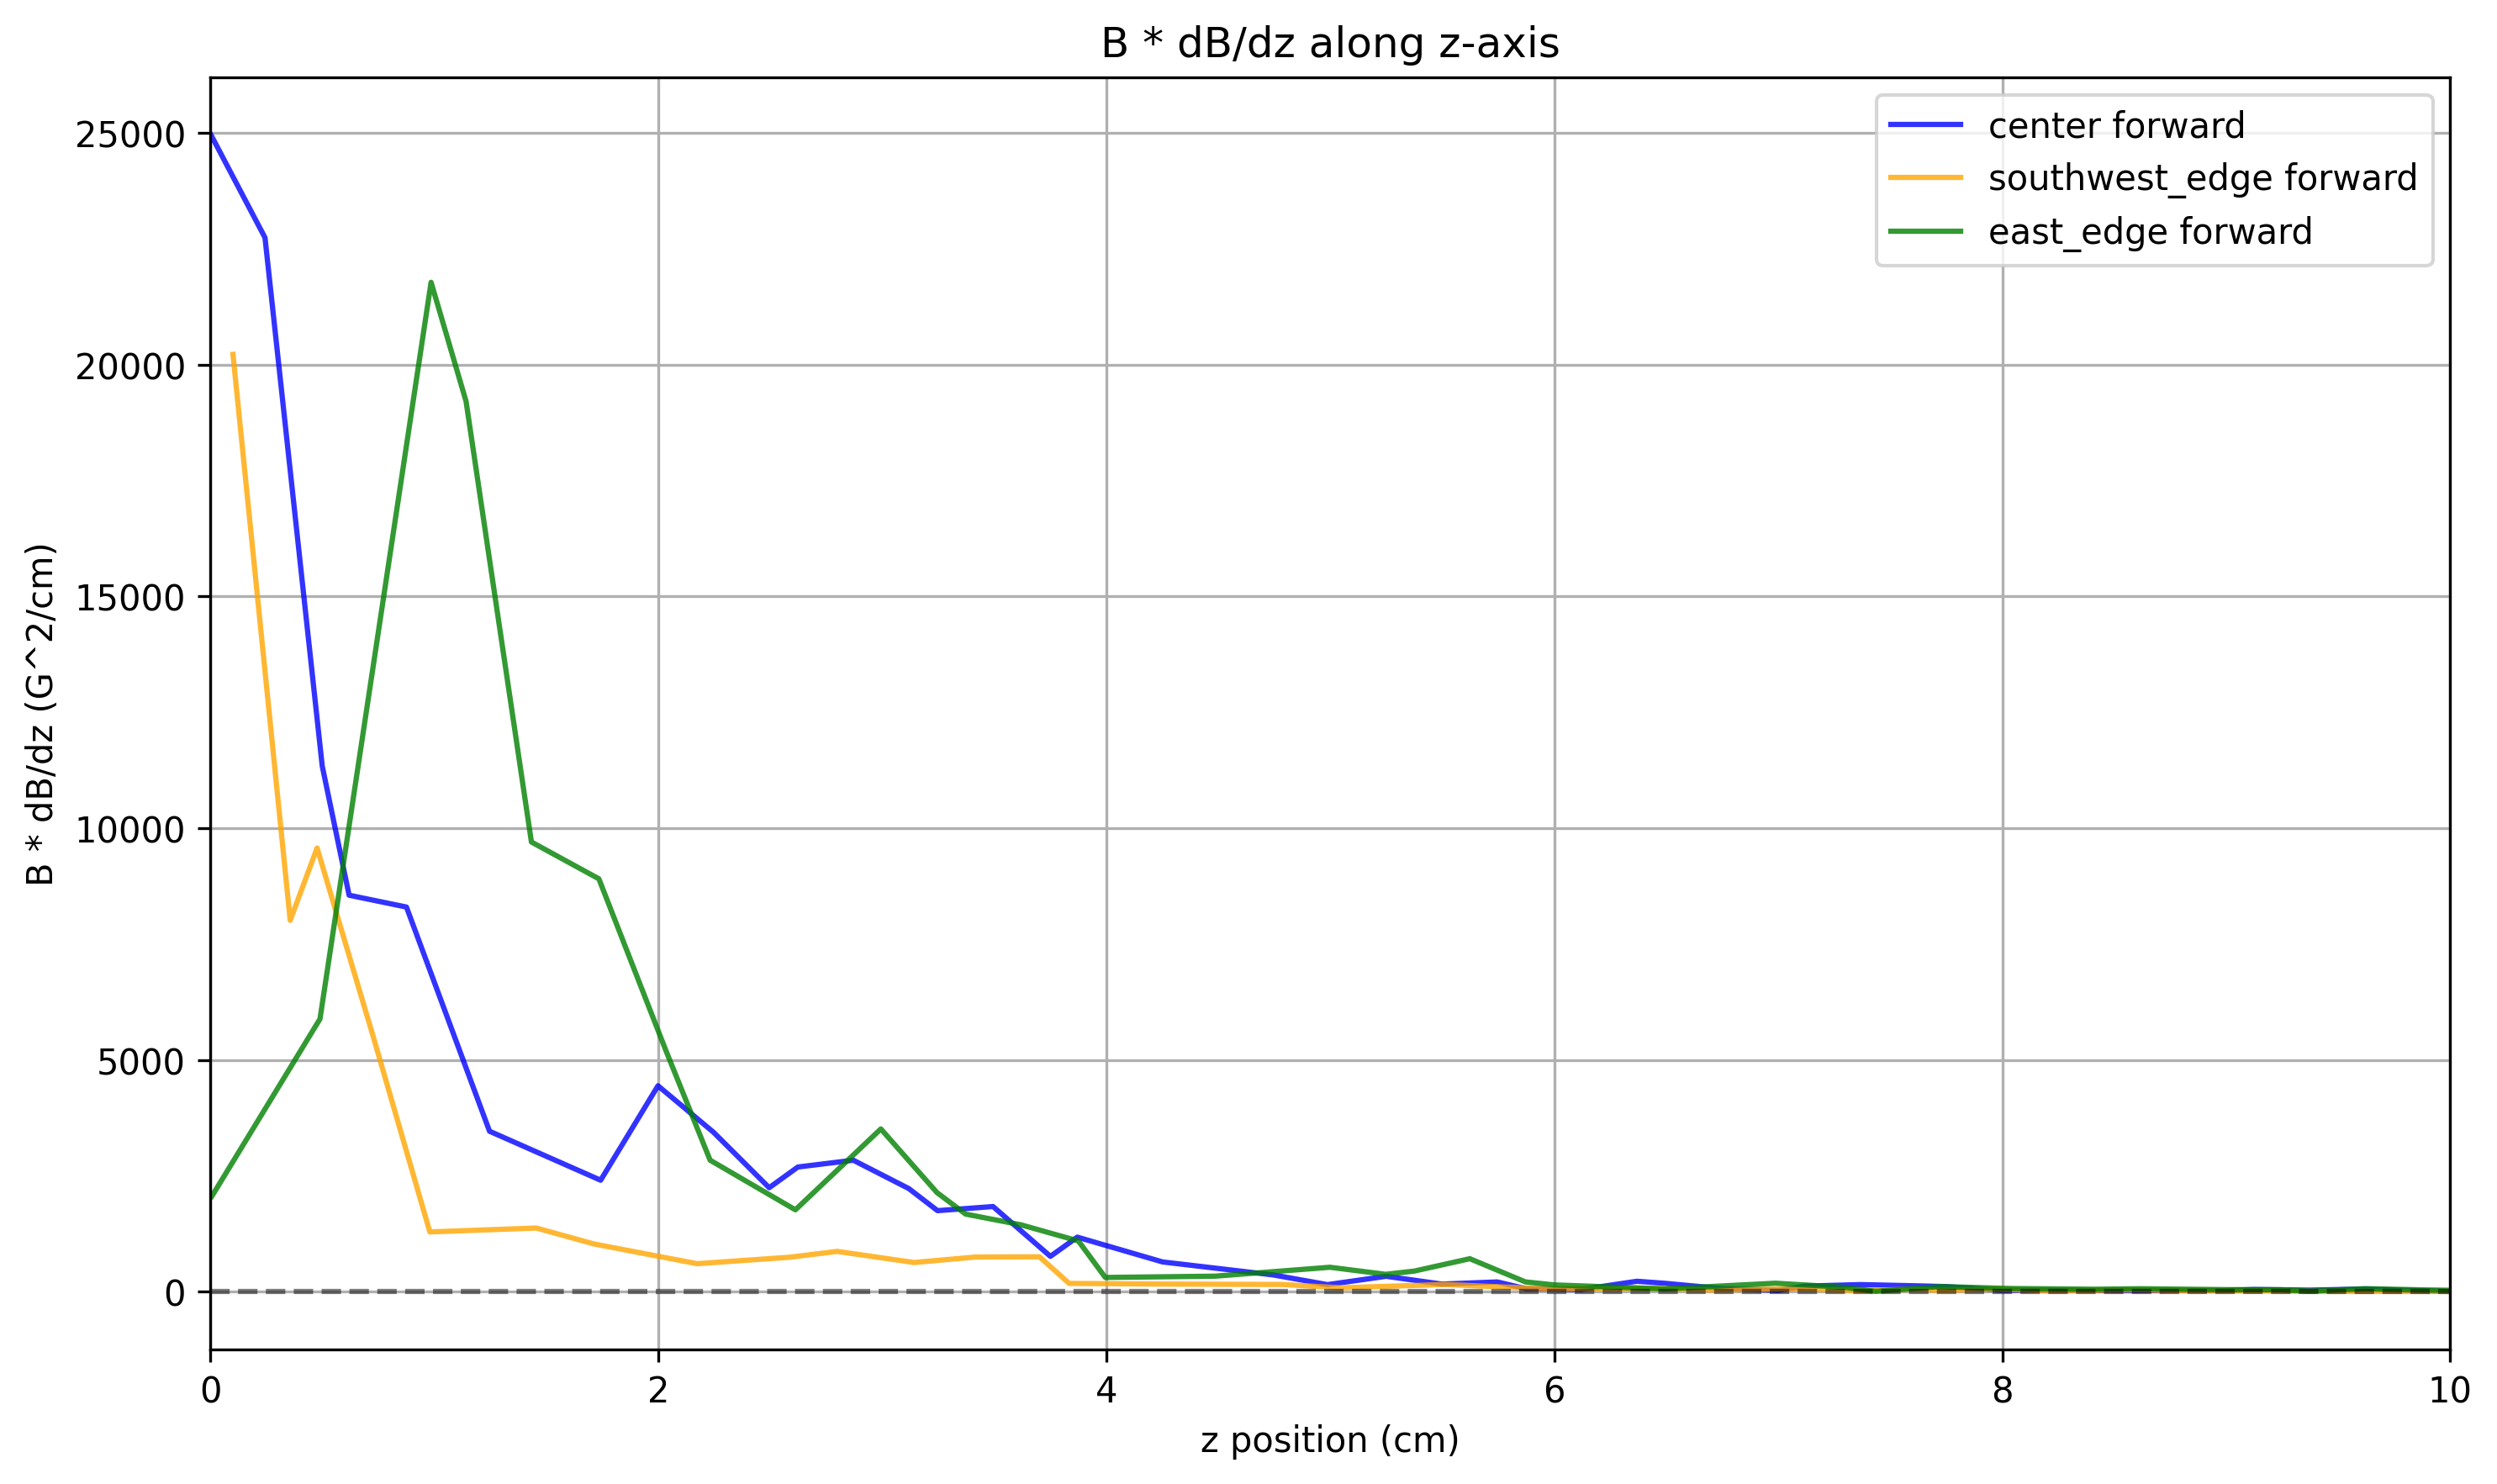
\includegraphics[width=0.90\textwidth]{Assets/BgradB.png}
	}
	
	\caption[Spatial magnetic gradients and $B\nabla B$ product]{Computed magnetic field gradients and the $B\nabla B$ product used for translational force characterization.}
	\label{fig:gradb_pair}
\end{figure}

In the translational experiment, the current applied to our solenoid was varied, and the magnetic field was measured in specific points within 7 to 8 cm away from the solenoid, this lead to a different results which are the points of equilibrium of the pendulum. These results are meaningful and will be used in section \ref{sec:res_labscale-Translational}. 

\begin{figure}[htb!]
	\centering
	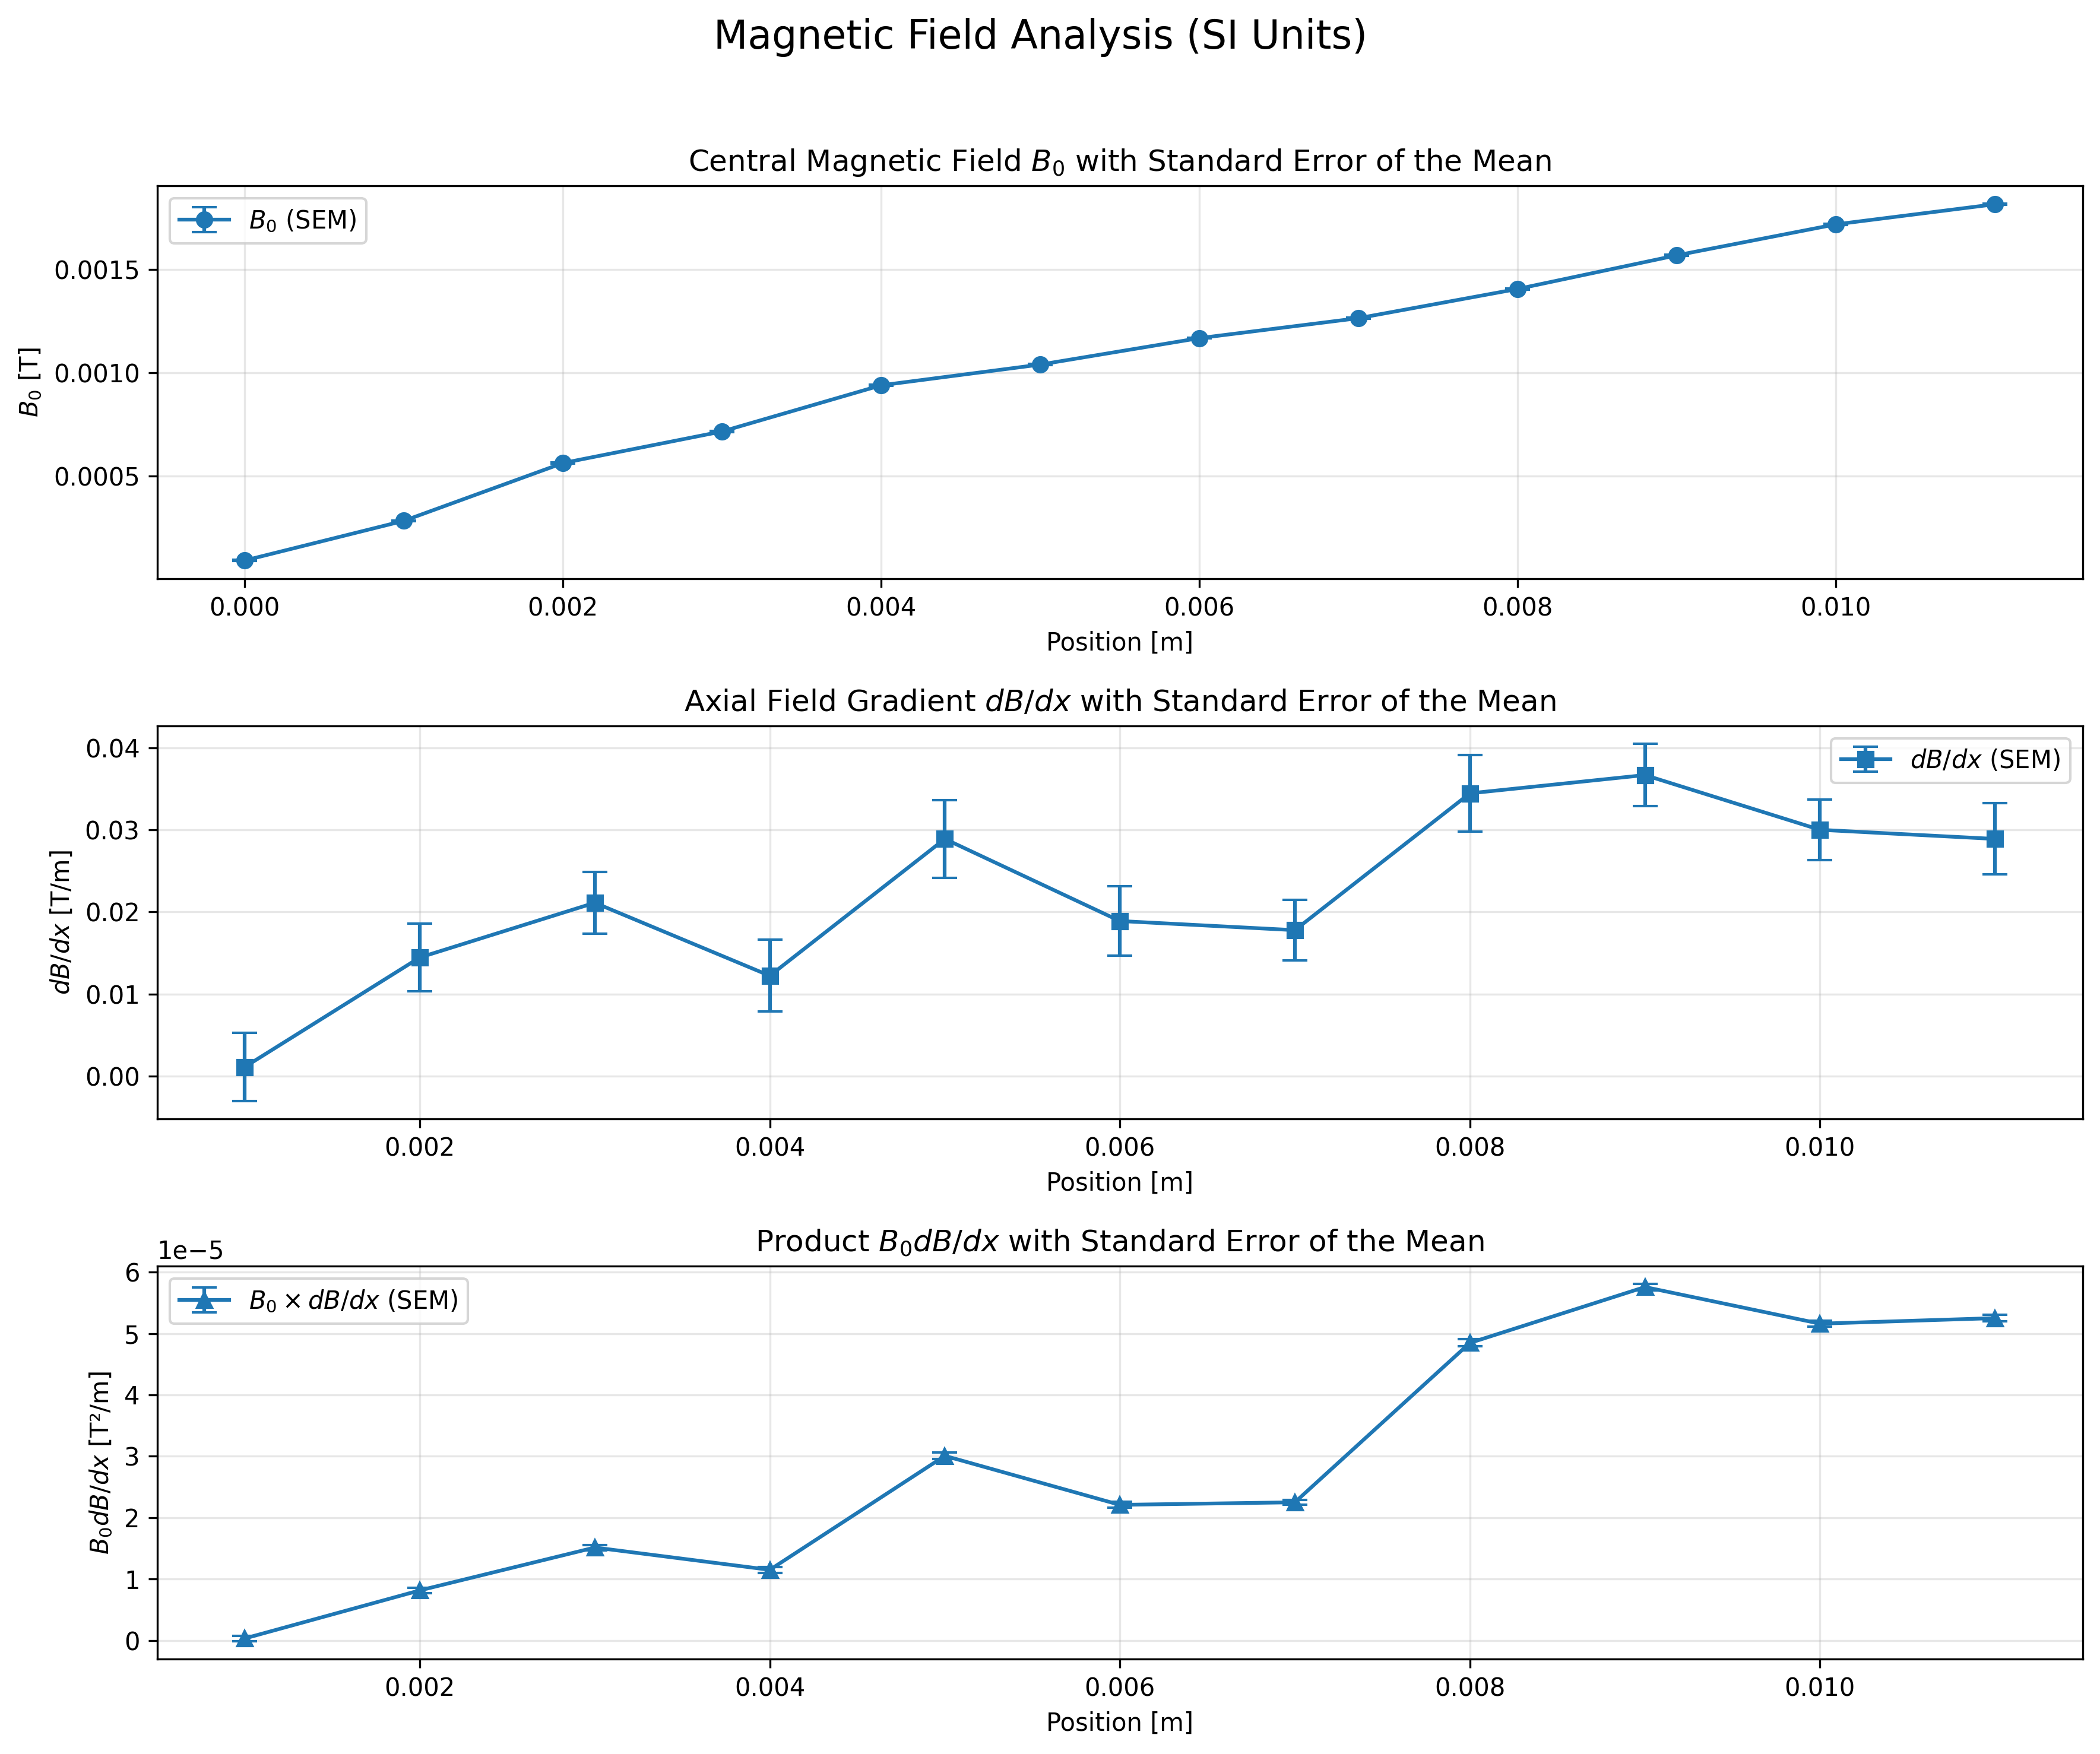
\includegraphics[width=0.9\textwidth]{Assets/magField_behavior_SI.png}
	\caption[Magnetic field behavior in SI units]{Central magnetic field $B_0$, axial field gradient $dB/dx$, and their product $B_0 dB/dx$ as functions of position along the magnet axis. All quantities are shown in SI units (Tesla, T/m, and T$^2$/m, respectively) with error bars representing the standard error of the mean (SEM).}
	\label{fig:EquilibriumPointsField}
\end{figure}

As the measurement of magnetic field was done by varying current and not distance the magnetic field plots looks different of that showed by Figures \ref{fig:bfield_time_z} and \ref{fig:gradb_pair}. Figure \ref{fig:EquilibriumPointsField} shows three plots, which corresponds to the three operations needed to make the field side of Equation \ref{eq:forFit}. As highlighted, in this instance the x-axis, position, refers to the position of the pendulum's end with respect of its gravitational equilibrium point, and each point was taken with a different current applied to the solenoid while the pole remained stationary.

\subsection{Mapping for 3T Siemens Magnetom\textsuperscript{\texttrademark} \gls{mri} scanner}




From the measurements of B and $\nabla$B the translational force experiment follows. The next section (\ref{sec:res_labscale-Translational}) shows the laboratory approach findings. After that, we evaluate the deflection angle in the clinic setting and talk about the significance of bringing this fixture to the clinic.

\section{Translational Force}
\subsection{Translational forces from a Laboratory scale magnet (up to 180 Gauss)}
\label{sec:res_labscale-Translational}

Figure \ref{fig:fit} shows a plot of the observed unitless displacement, [tan($\alpha$)] against the magnetic field properties (B$\nabla$B) in $T^2/m$, which were determined from mapping the magnetic field. Figure \ref{fig:curve_fit_plot} is a representation of Equation \ref{eq:forFit}, it shows a linear fit with a slope of 160.3186 $\pm$ 8.2631 and intercept 0.0160 $\pm$ 0.003. Figure \ref{fig:residuals_plot}, shows the residuals for the linear fit suggesting this fit is appropiate.

\begin{figure}[htb!]
	\centering

	\subfigure[Curve fit of measured pendulum deflection vs. applied magnetic force.\label{fig:curve_fit_plot}]{
	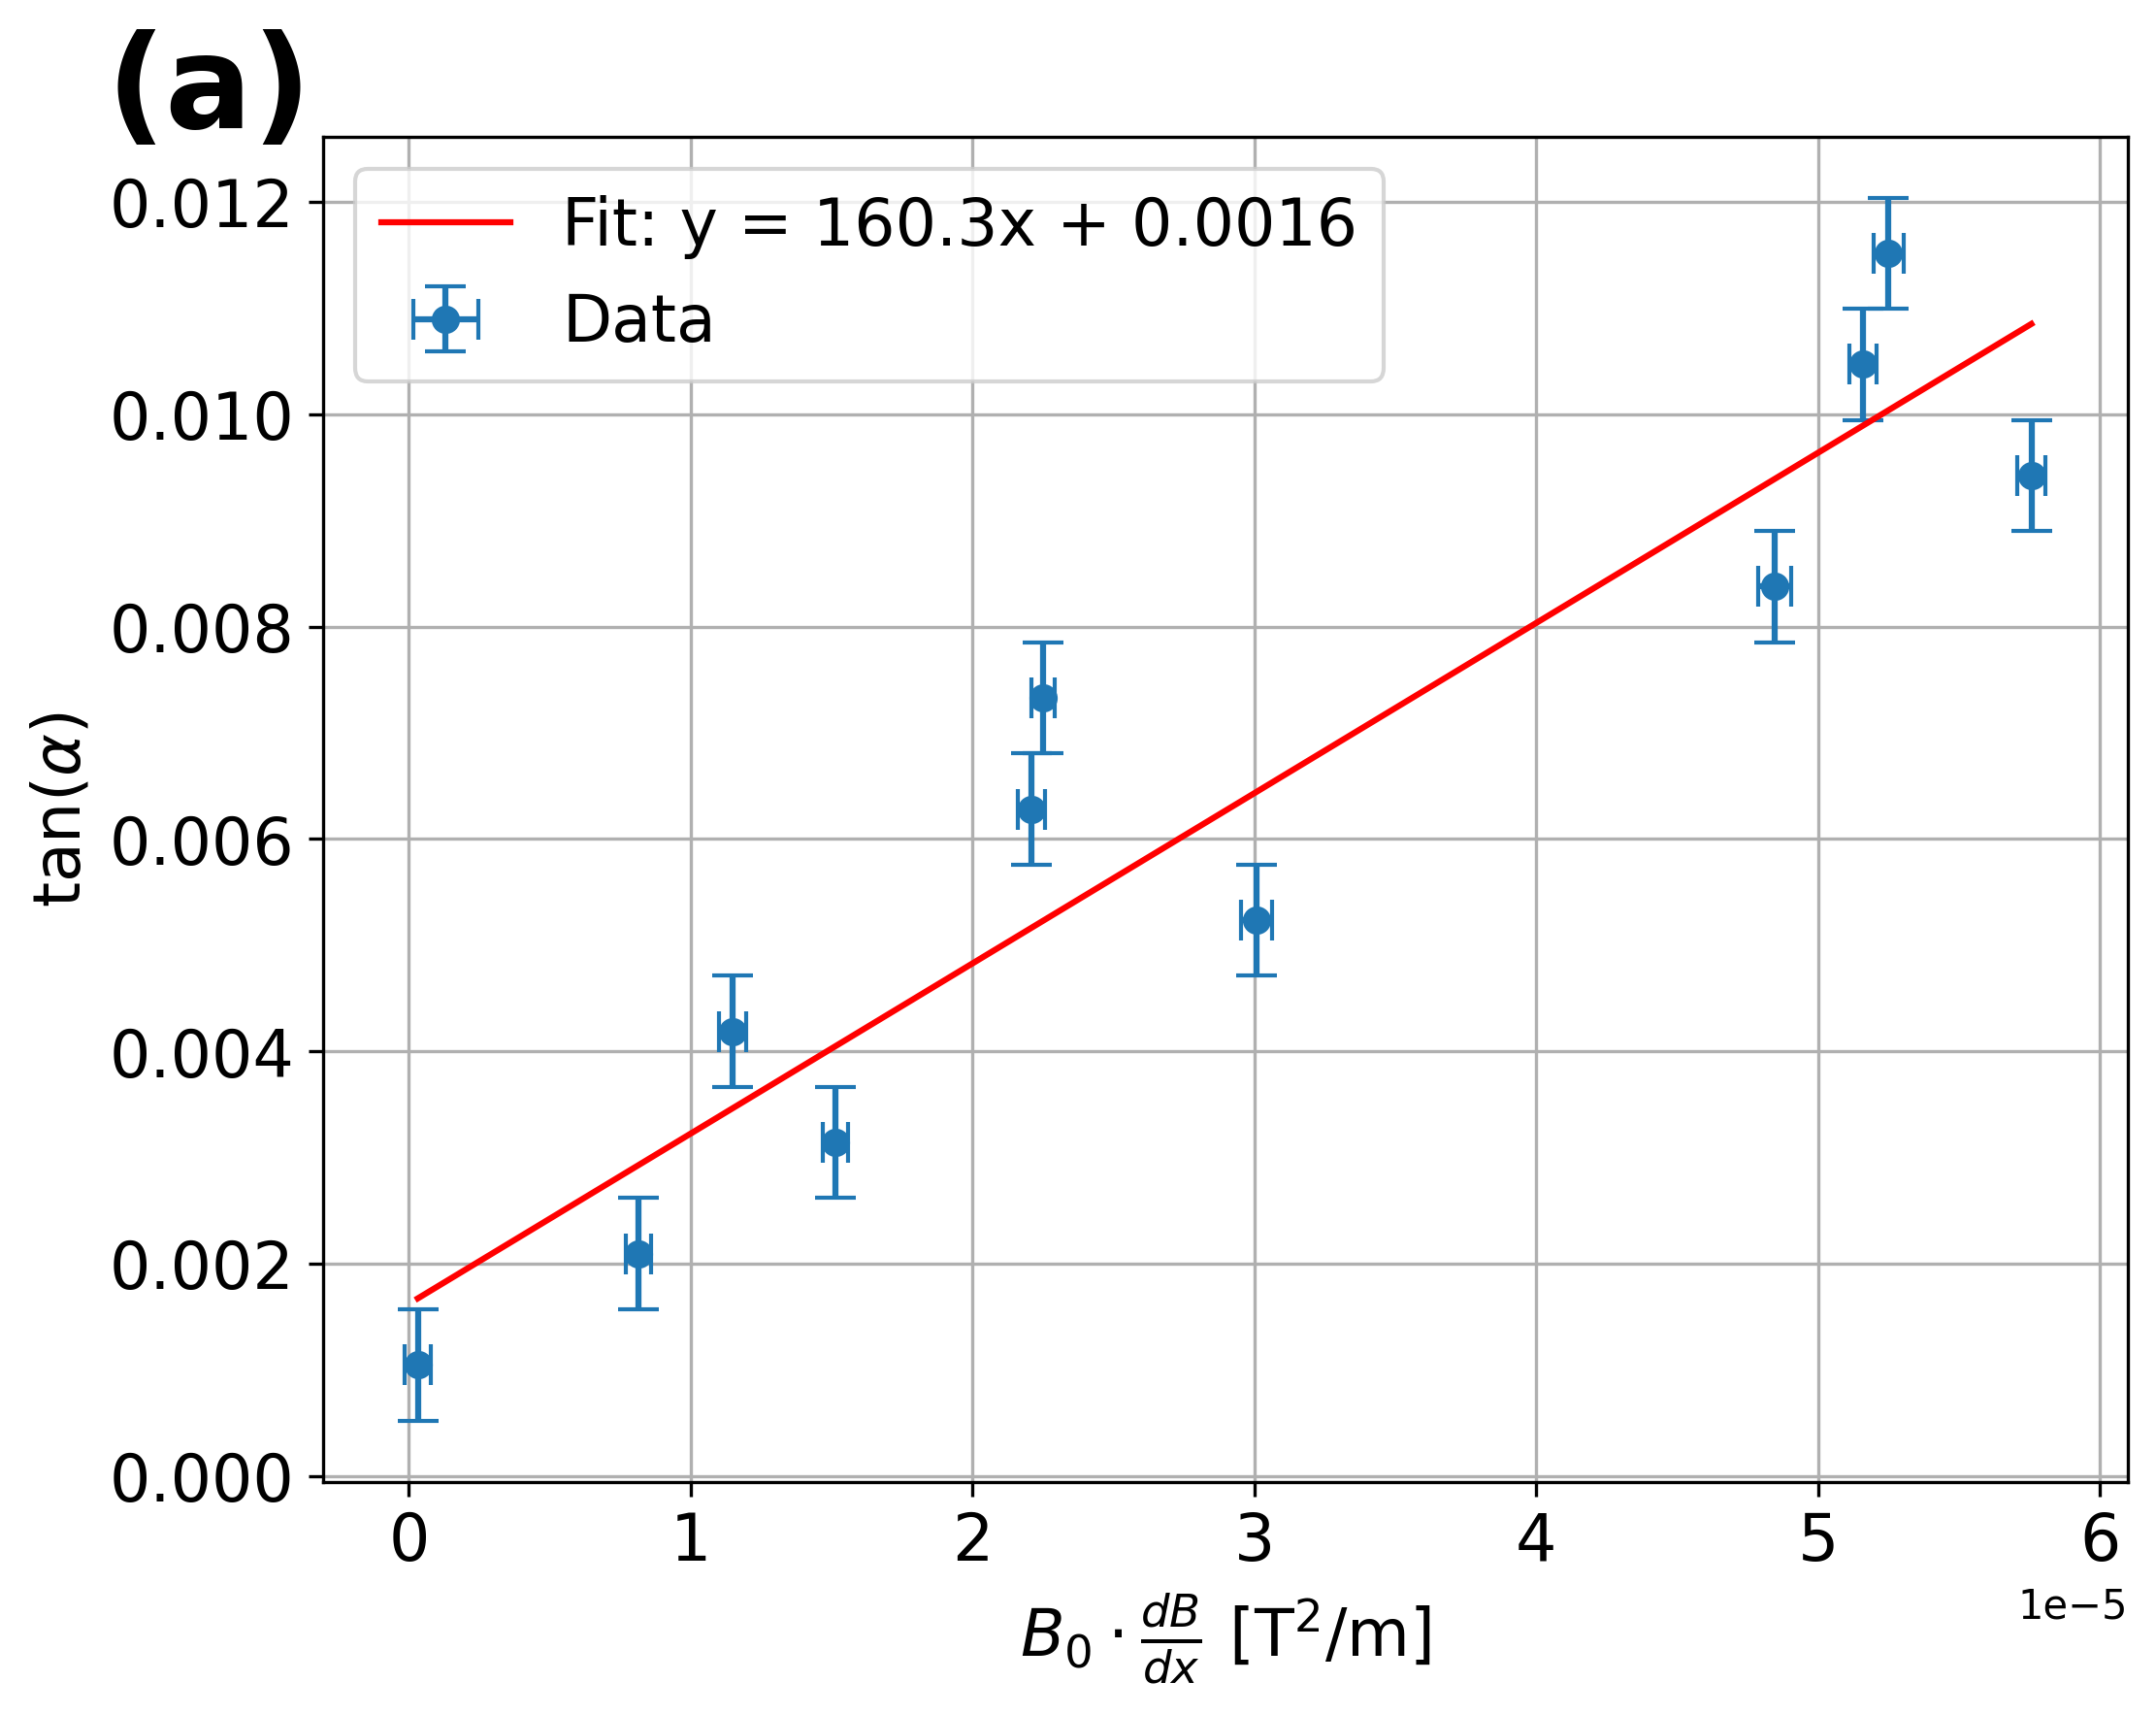
\includegraphics[width=0.9\textwidth]{Assets/curve_fit_plot.png}
	}
	\hfill
	\subfigure[Residuals from linear fit of $\tan(\alpha)$ vs. $B_0 \cdot \frac{dB_0}{dz}$. Error bars indicate propagated uncertainties.\label{fig:residuals_plot}]{
		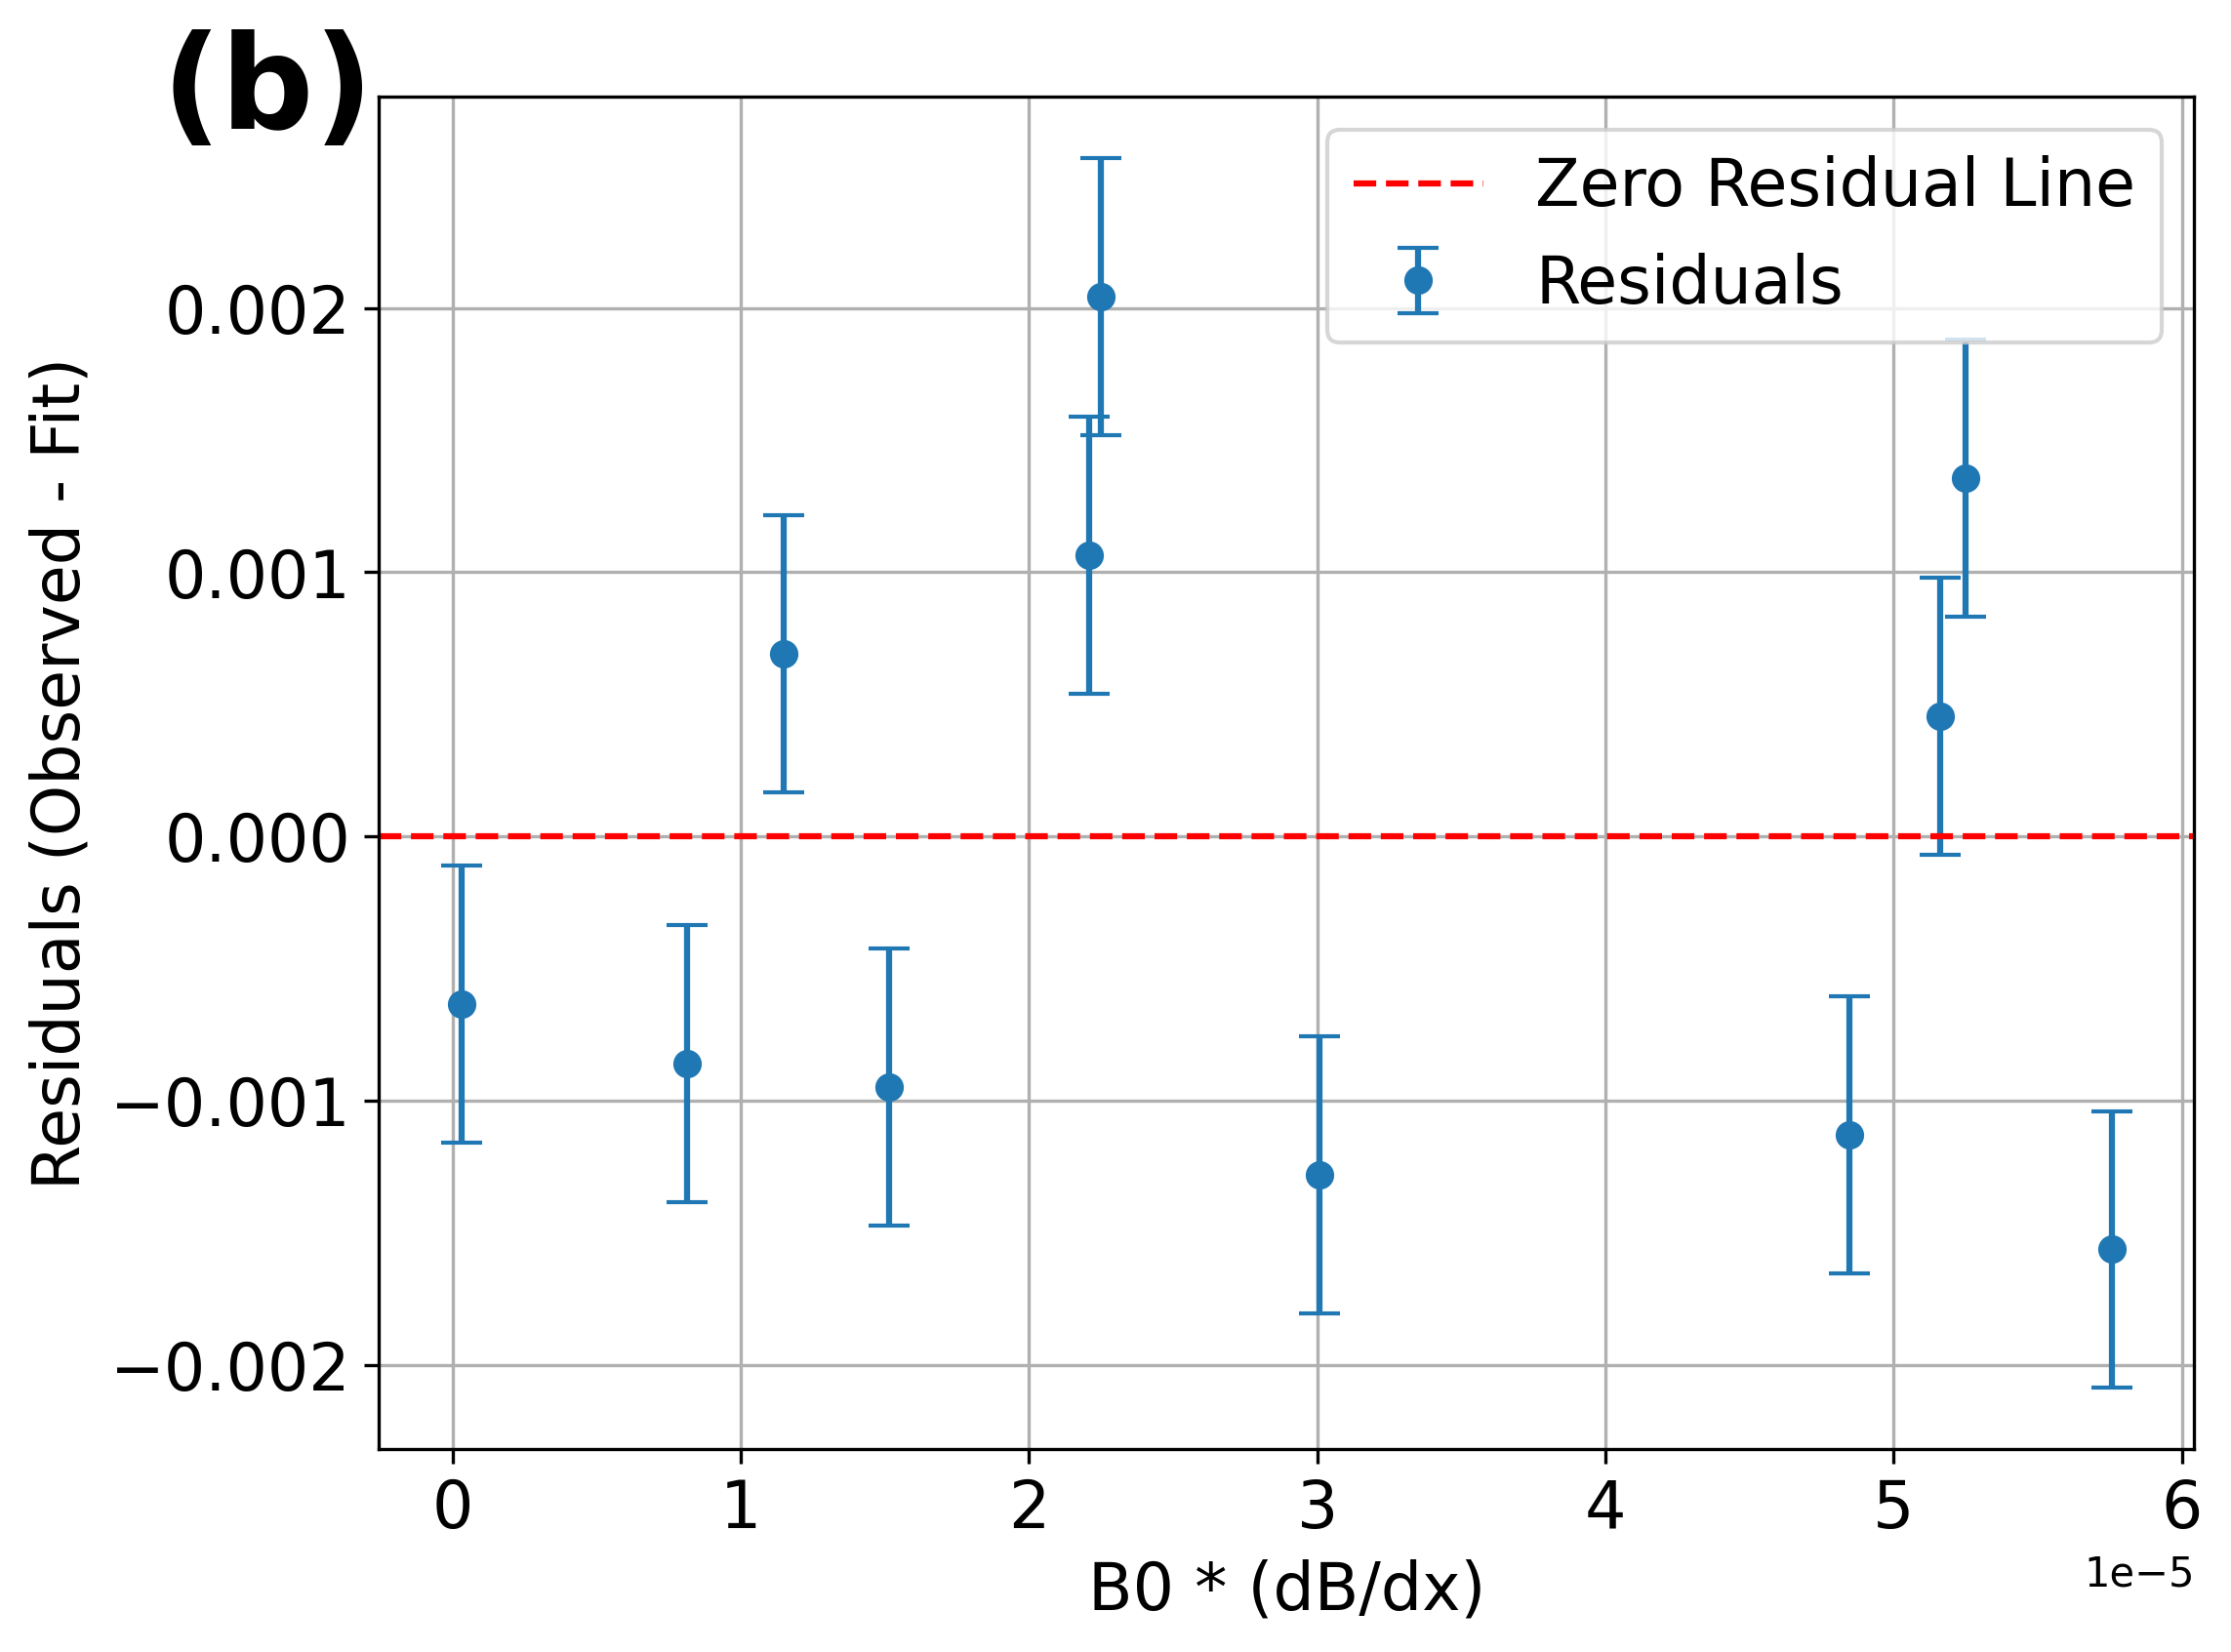
\includegraphics[width=0.9\textwidth]{Assets/Residuals_Plot.png}
	}
	\caption[Residuals and curve fit comparison]{: (a) residuals from the linearized fit, and (b) fitted curve against the measured data points.}
	\label{fig:fit}
\end{figure}

 Following Equation \ref{eq:forFit}, it can be quickly inferred that the magnetic susceptibility of the our sample is given by 
 
 \begin{equation}
 \chi = m (\mu_0 \rho g)  
 \end{equation}

\noindent where $m$ is the slope found with Figure's \ref{fig:curve_fit_plot} fit, $\mu_0$ the vacuum permittivity, $\rho$ the material's density and $g$ gravity. Sample characteristics are shown in Table \ref{tab:subjectProp}. This table shows the measured quantities, length, diameter and mass with its calculated relevant parameters (Volume, Density [$\rho$] and magnetic susceptibility [$\chi$])


\begin{table}[htb!]
	\centering
	\caption[Properties of the magnetic subject – experimental and theoretical values]{Measured and calculated characteristics of our magnetic subject depicted in Figure \ref{fig:ferrobject}}
	\begin{tabular}{lcc}
		\hline
		Property & Value & Unit \\
		\hline
		Length & $6.00 \pm 0.01$ & mm \\
		Diameter & $3.00 \pm 0.01$ & mm \\
		Mass & $0.3648 \pm 0.0001$ & g \\
		\hline
		Volume & $(4.241 \pm 0.029) \times 10^{-8}$ & m$^3$ \\
		Density & $8601 \pm 59$ & kg/m$^3$ \\
		Mass magnetic susceptibility [$\frac{\chi}{\rho}$] & $(2.01 \pm 0.05) \times 10^{-3}$ & m$^3$/kg \\
		Magnetic susceptibility (unitless) & $17.29 \pm 0.12$ & \\
		\hline
	\end{tabular}
	\label{tab:subjectProp}
\end{table}

Importantly, from Figure \ref{fig:curve_fit_plot}, tan($\alpha$) is in the range of 0.002 to 0.012. From Equation \ref{eq:deflectionAngle}, and according to ASTM 2052 \cite{astmF2052}, the force ratio threshold for MRI safety indicates 1 or, equivalently, a deflection angle of 45$^\circ$ putting our measurements way bellow that threshold for our lab simulation. In the clinic, the magnetic field is about 1.7 hundred times bigger than what we found in our lab. With samples being paramagnetic, roughly 1 million to 10 million times smaller than what we found here.


\subsection{Translational forces observed in a 3T Siemens Magnetom\textsuperscript{\texttrademark} \gls{mri} scanner}

\FloatBarrier


The last piece of the assessment is the torque measurement. This time, laboratory work includes sensor calibration leading into in-lab measurements, while clinical observations remain unclear.

\section{Torque} 
Parallel to section \ref{sec:metsTorque}, we split this section into three pieces, first the results yielded by our sensor-circuit system calibration, then the in-lab work and at last the clinical findings.

\subsection{Sensor Calibration}
\label{sec:calResult}

% ============================================================
% APPENDIX E -- Torque Sensor Calibration Additional Results
% ============================================================

This appendix presents supplementary results from the torque sensor calibration process described in Section~\ref{sec:sensorCal}. The aluminum-based sensor was selected for all reported measurements based on its consistency and sensitivity relative to the other candidate materials. The figures here document the calibration trials for the glass and clear plastic sensors, which showed insufficient linearity and voltage range for reliable use. Together these results justify the sensor selection and positioning choices reported in Chapter~\ref{ch:matsNmets} and use for results presented in Chapter \ref{ch:results}.

The sensor calibration consisted in incrementally adding weight to our sensor as described in section \ref{sec:sensorCal}. The strain sensors studied included clear plastic, aluminum, and glass. Each sensor was tested for linearity voltage vs. weight up to 800 mg. Figure \ref{fig:rods5n7} shows calibration plots for two of the trials done. (a) The glass sensor showed some linearity, but small mean voltage range of operation even at max weight. The slope found for each fit is too different and non reproducible. (b) The clear plastic sensor showed stiffer,  showing better slope trend consistency but still being too uncertain.

These results demonstrated that these sensors were unreliable, and characterized by unpredictable changes in voltage when weight was applied. Additionally, both sensor had a sub-millivolt range, ineffective for measurements. These two rods were the thickest of all available rods in Table \ref{tab:rods}. The observed behavior is expected as explained by Equation \ref{eq:force_to_voltage}.


\begin{figure}[htb!]
	\centering
	
	\subfloat[\label{fig:glassRod5}]{
		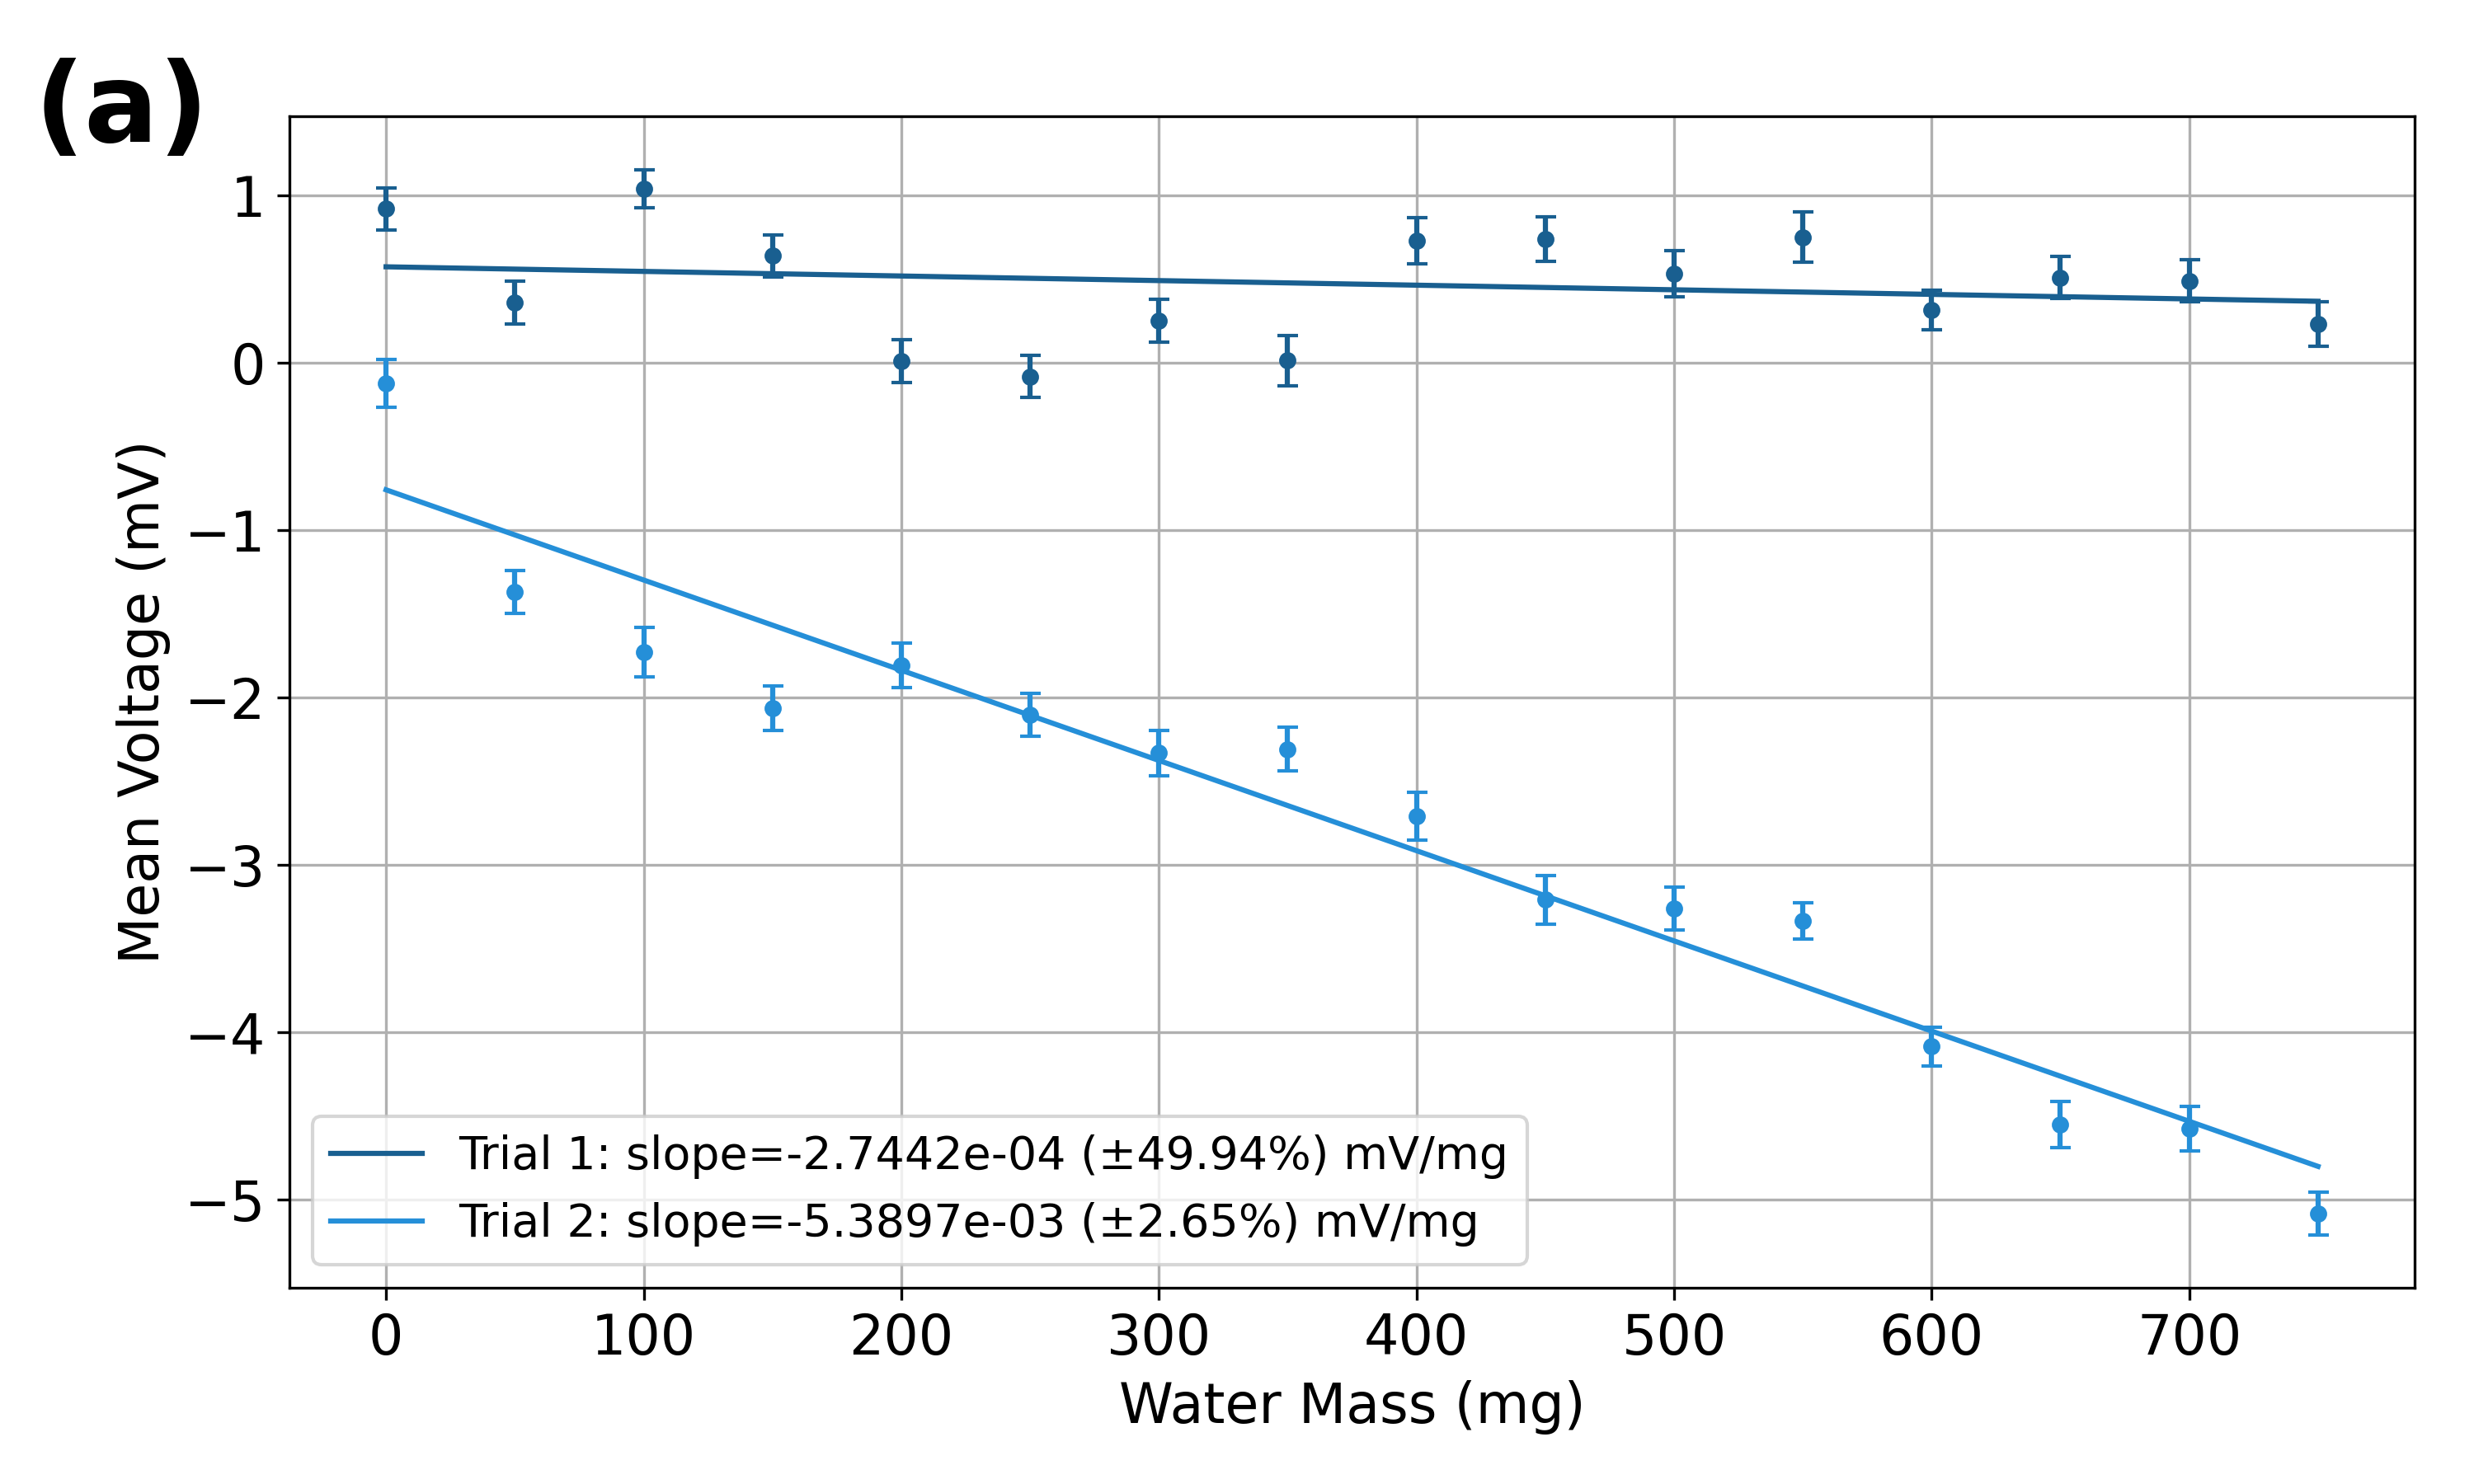
\includegraphics[width=\textwidth]{Assets/glass_fit.png}
	}
	\hfill
	\subfloat[\label{fig:clearRod7}]{
		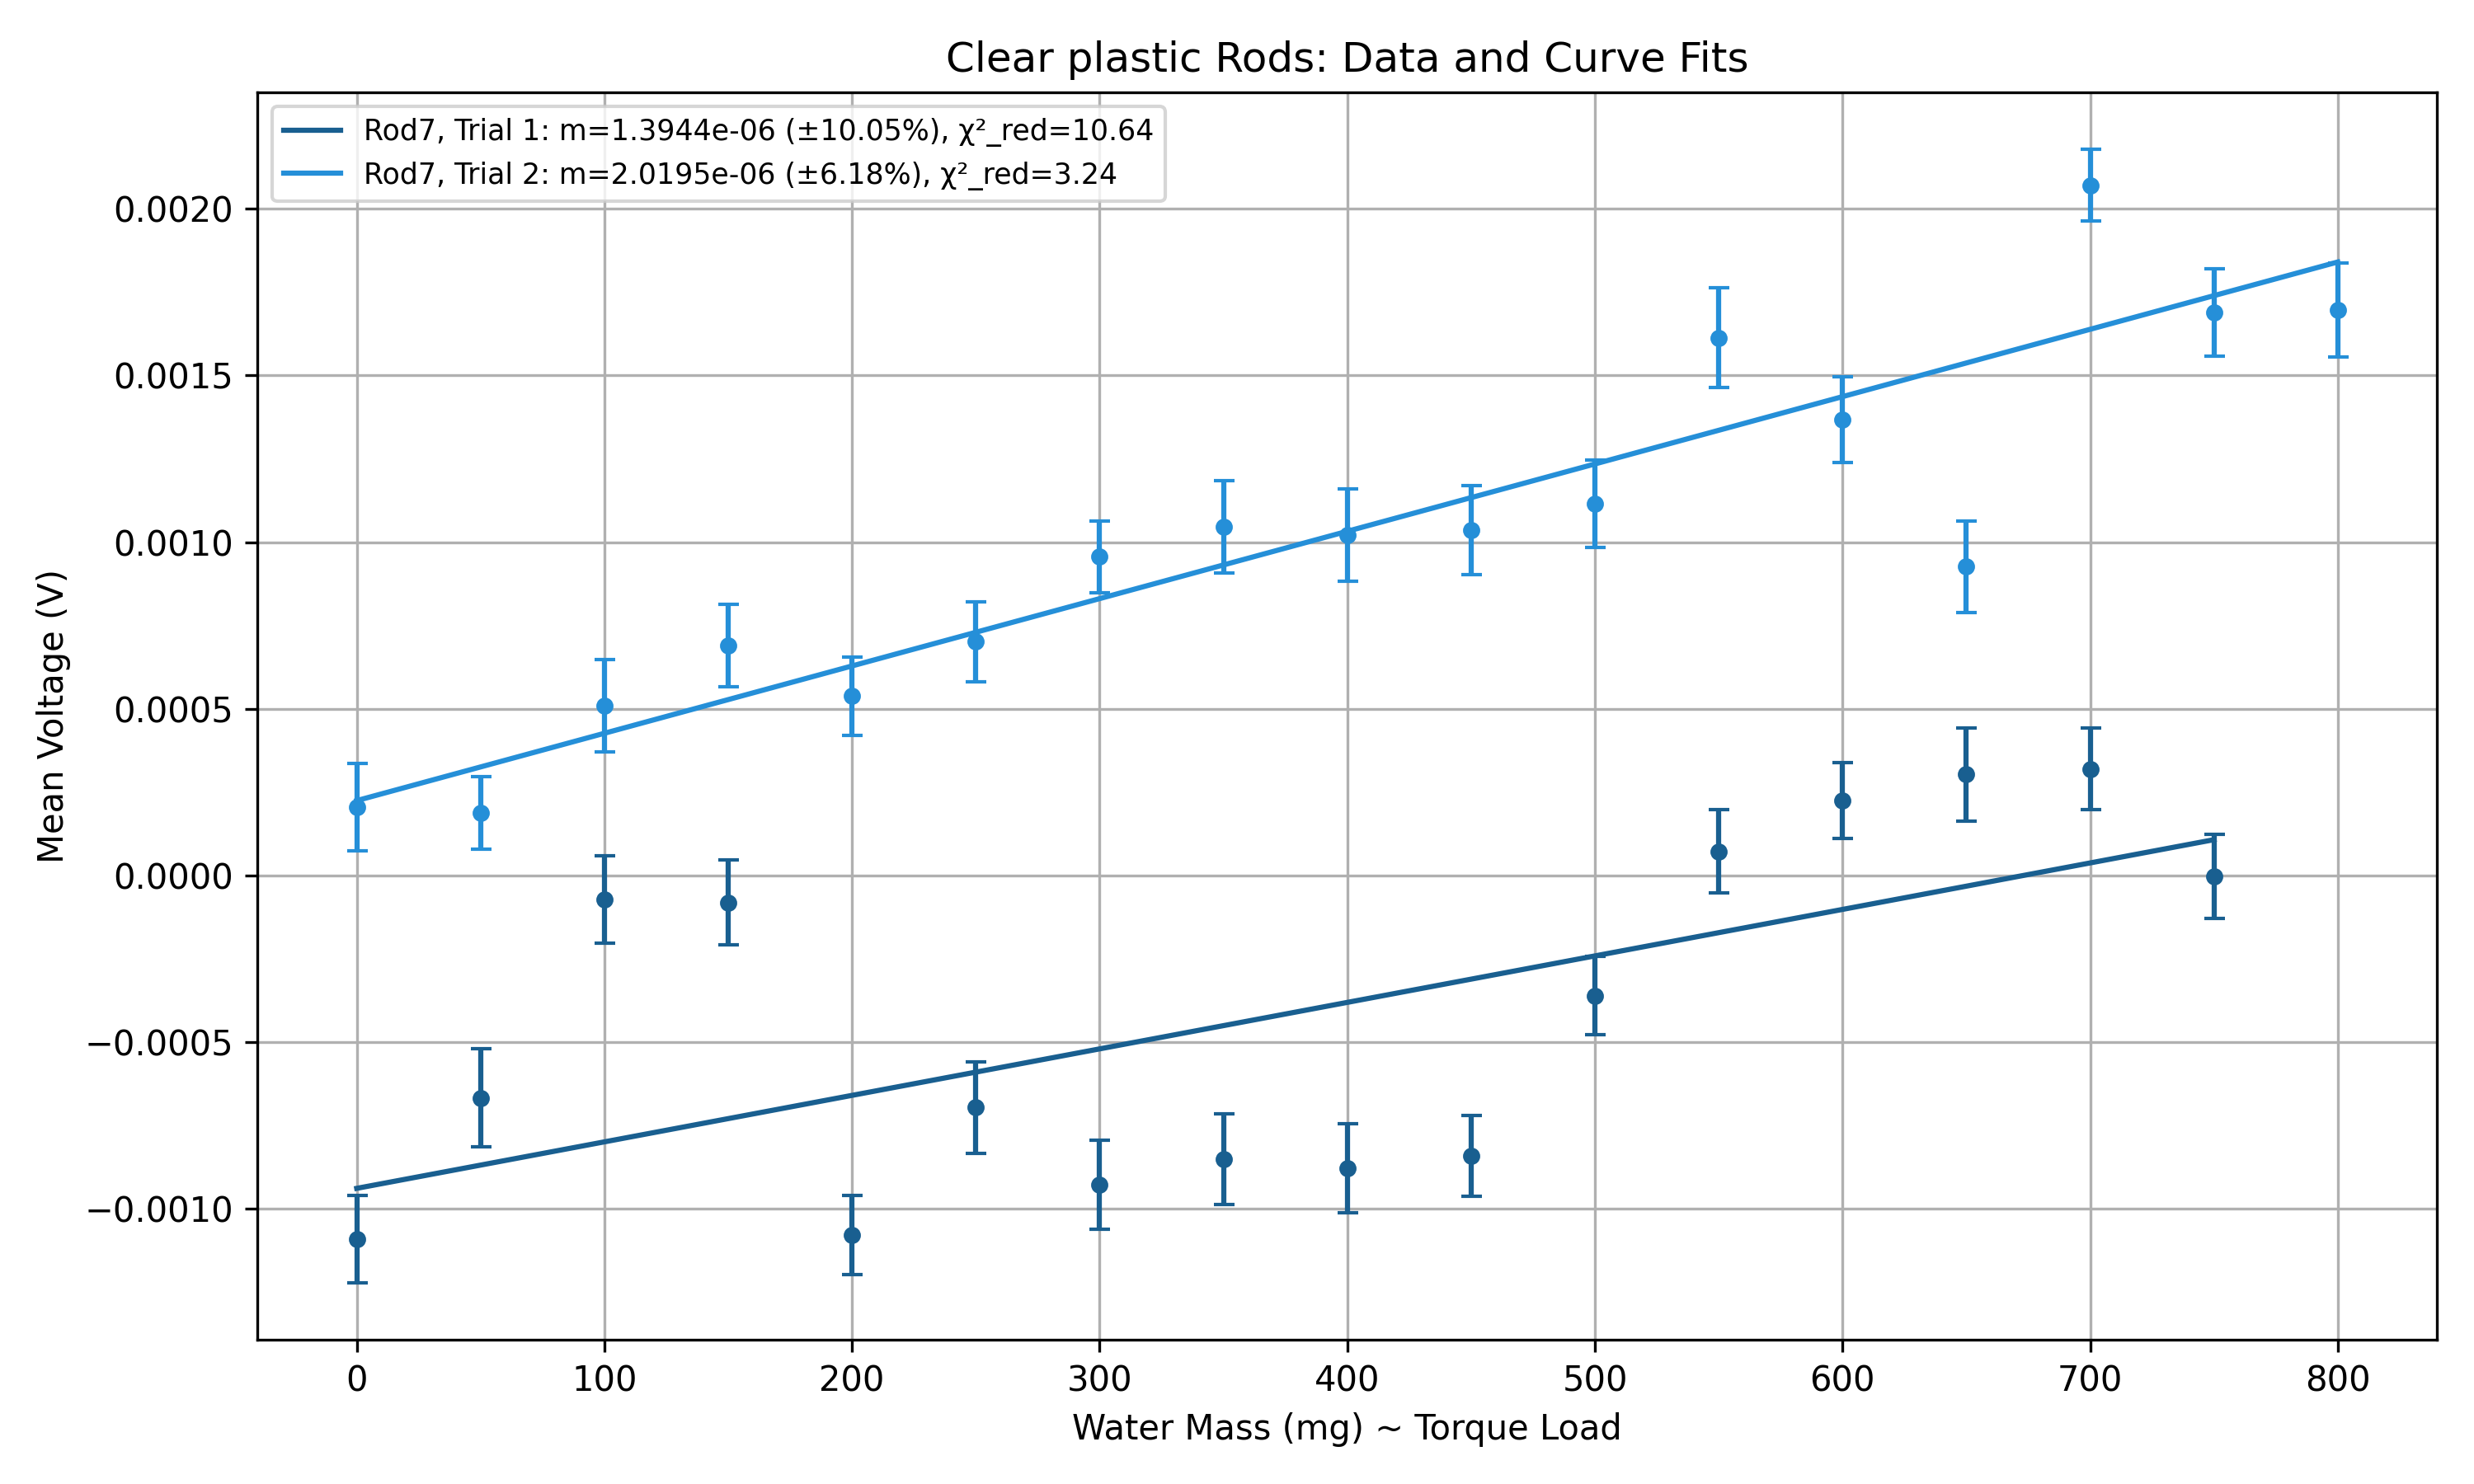
\includegraphics[width=\textwidth]{Assets/clear_plastic_fit.png}
	}
	\caption[Calibration trial results for low-torque rods showing poor sensor response]{Trial examples for Rods 5 and 7. Both of them showed inconsistency across trials showing minimal to no change in voltage with weight added. (a) Voltage readings for Rod5 (Glass) with up to 750 mg of water in increments. (b) Voltage readings for Rod7 (Clear Plastic) with up to 800 mg of water in increments.}
	\label{fig:rods5n7}
\end{figure}

In contrast the aluminum rods, 2 and 3, showed a clear linear trend along all trials and measurements (Figure \ref{fig:scaleCalb} ). This plot features three different sensor rotation configurations (Fig \ref{fig:cantileverConfigs}). Either 0$^\circ$ or 180$^\circ$ gave maximum deformation of the strain gauges, while 90$^\circ$ was ineffective.

\begin{figure}[htb!]
	\centering
		\subfloat[\label{fig:linearfitAlrods}]{
		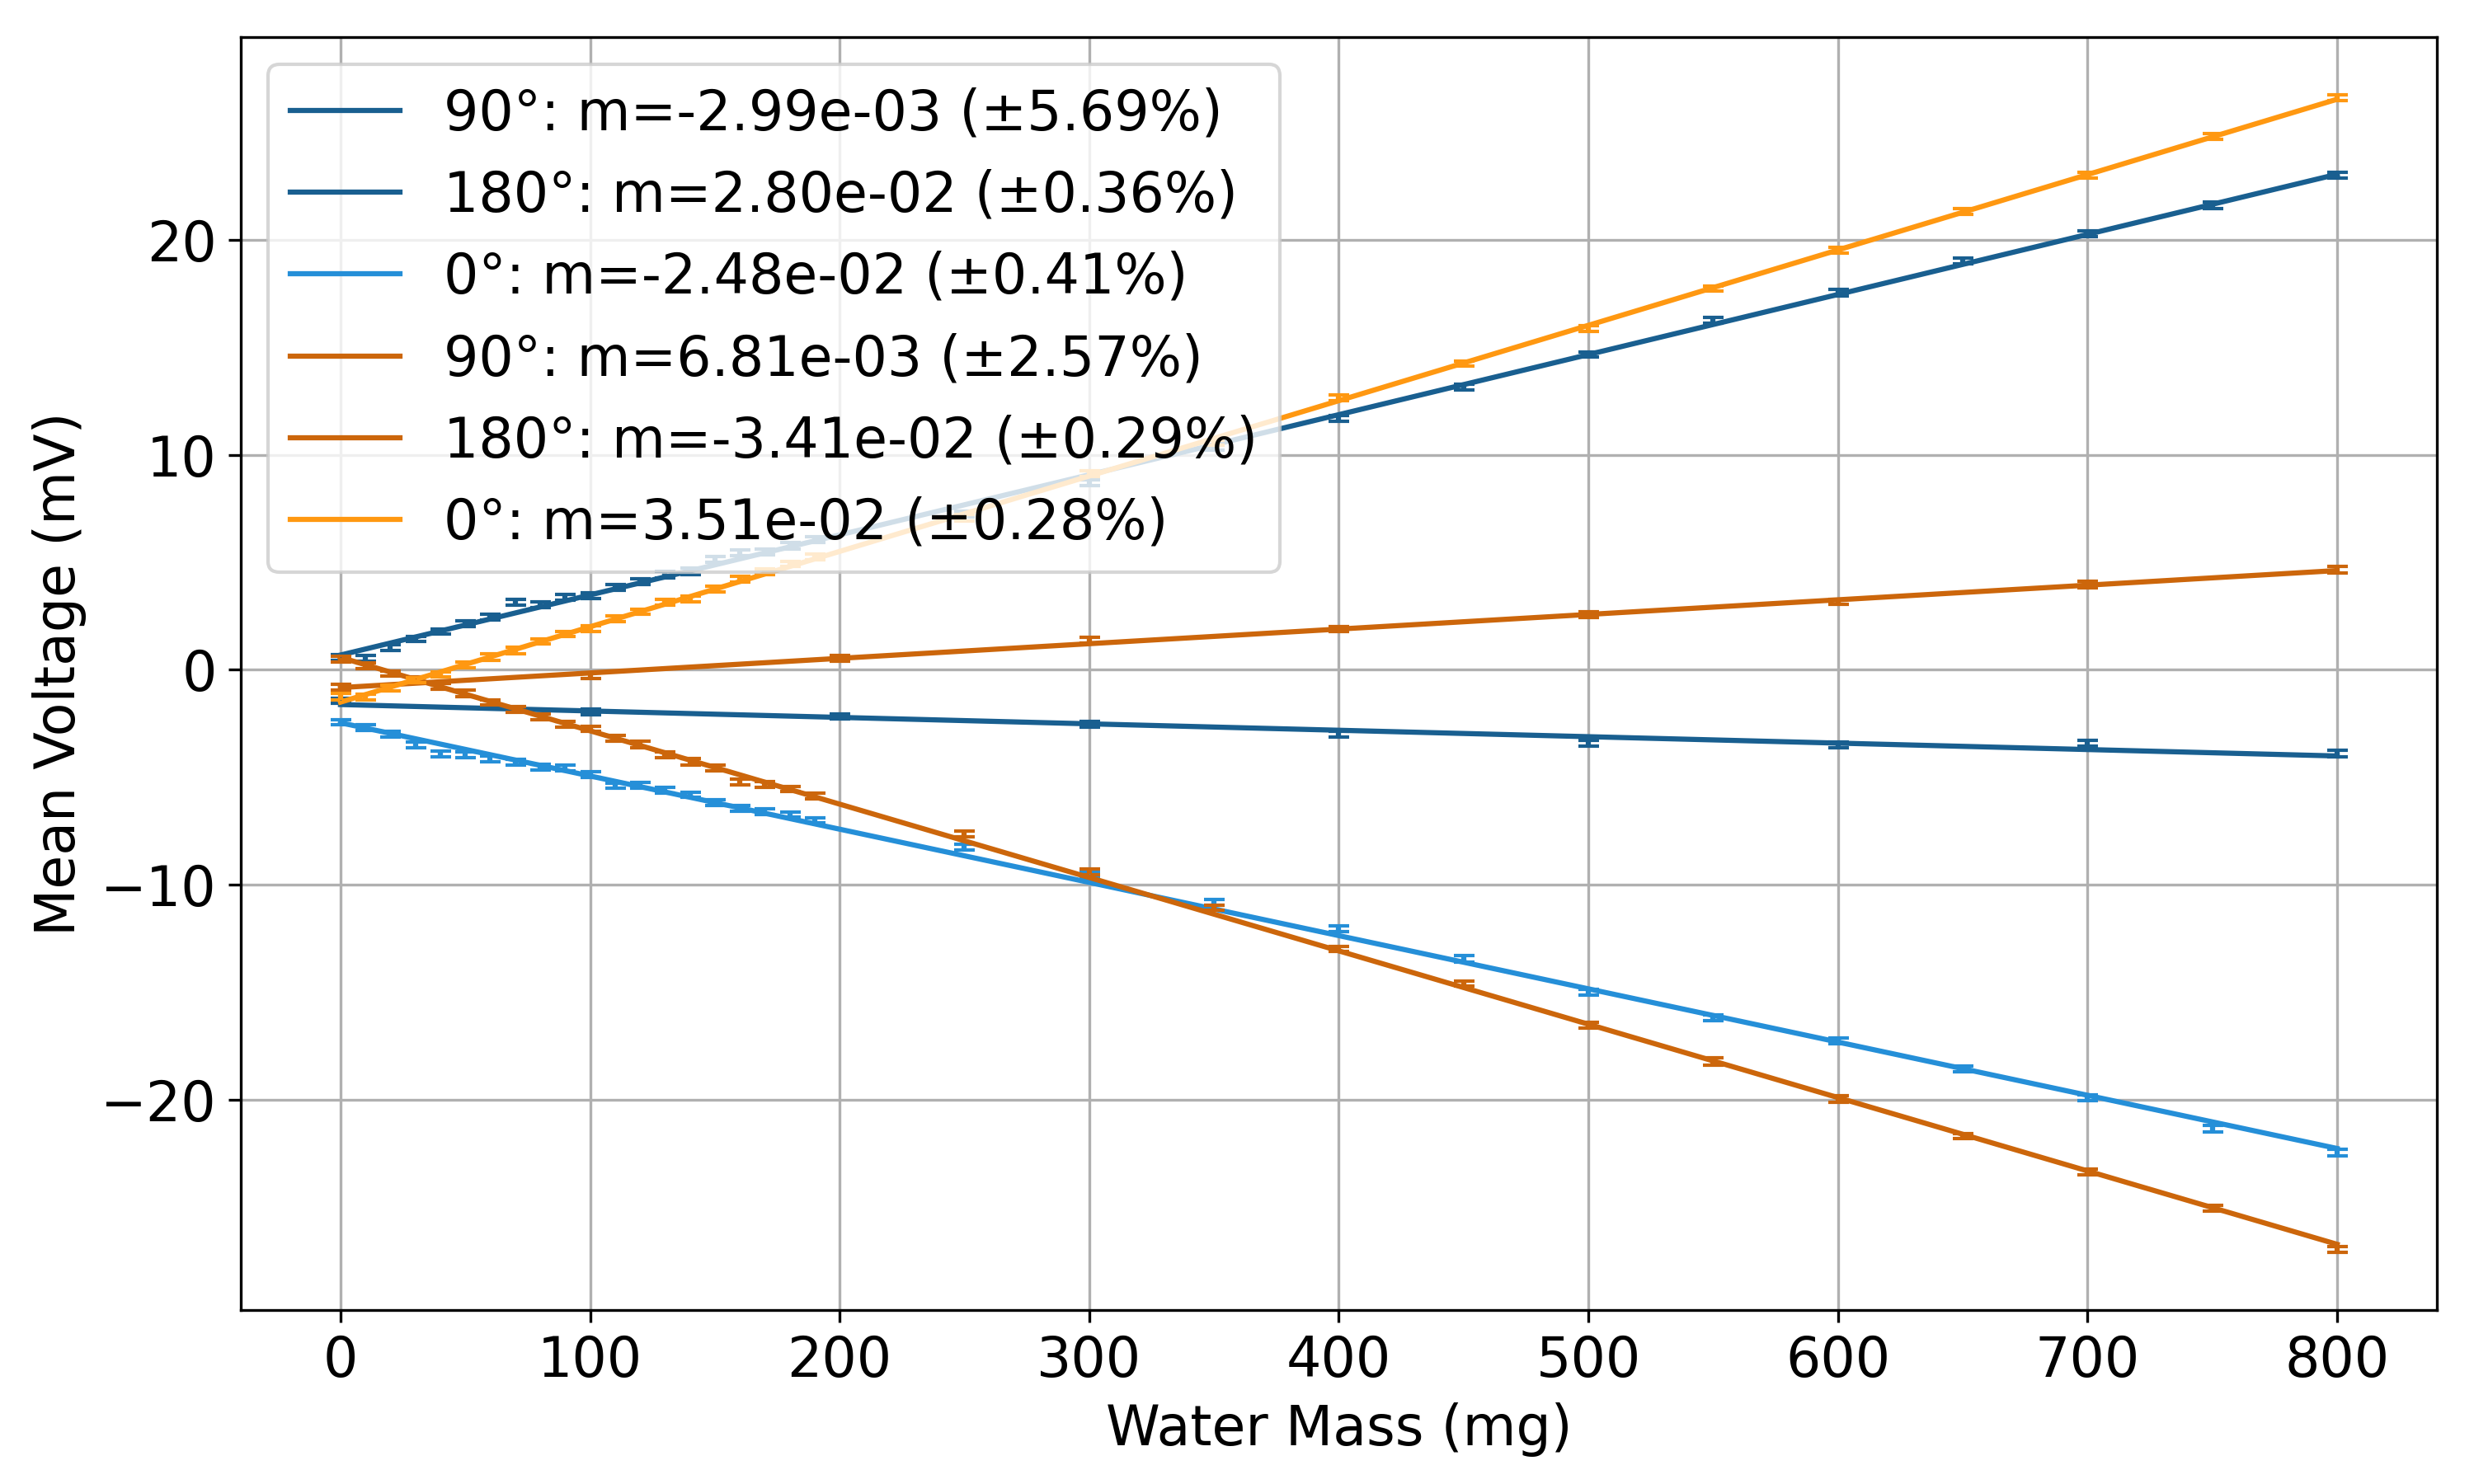
\includegraphics[width=0.95\textwidth]{Assets/al_fit.png}
	}
	\hfill
		\subfloat[\label{fig:cantileverConfigs}]{
		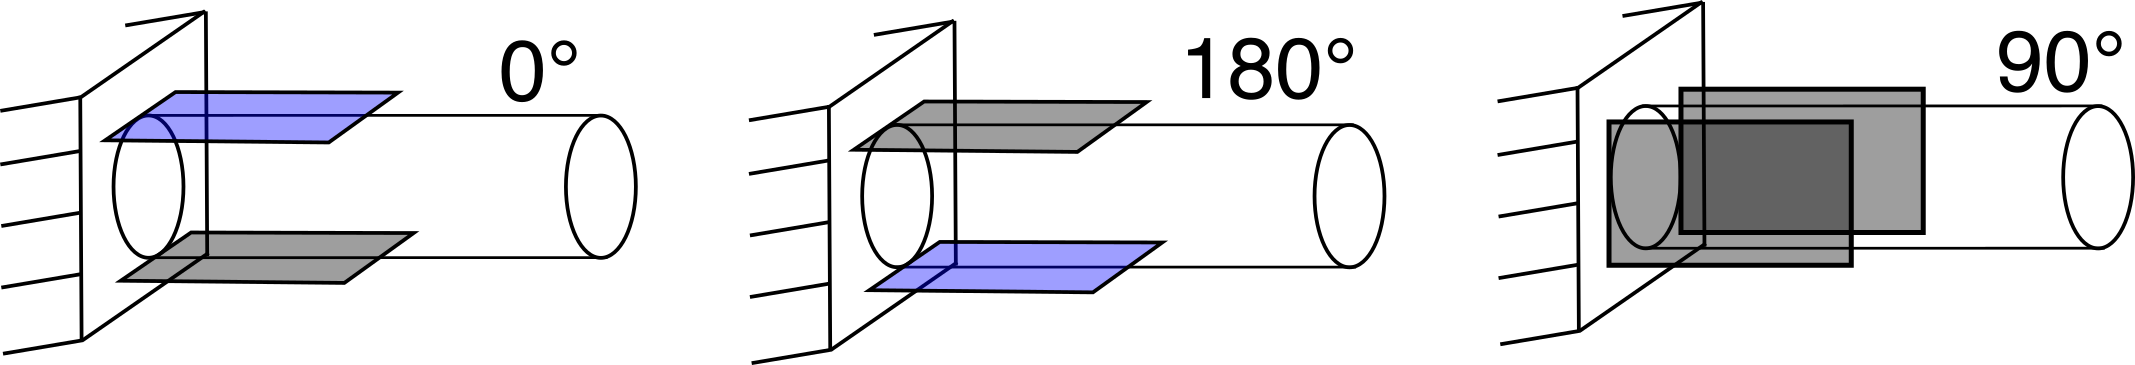
\includegraphics[width=0.85\textwidth]{Assets/calConfigs.png}
	}
	\caption[Orientation Response of cantilever sensor during calibration.]{Linear fits show consistent response across orientations, confirming the reliability of the lab-built sensor. (a)Calibration curves for two aluminum (AL) rods in three different orientations. (b)Three configurations tested, 0$^\circ$ and 180$^\circ$ are equivalent but flip voltage sign with respect of each other. 90$^\circ$ gives less sensibility as strain gauges does not bend in the proper axis.}
	\label{fig:scaleCalb}
\end{figure}

From these results, we used rod 3 oriented in either 0 or 180 degrees, since it showed remarkable consistency across calibration trials. Focusing on the weight range(0 to 200 mg), we found similar slopes in repeated calibrations over a period of one week.

Figure \ref{fig:posAndHeight} shows two lines, along the lever arm 90 and 50 mm ($r$) away from the rotation axis position. On the x-axis position along the sensor length measurements demonstrated greater sensitivity for greater distances from the strain gauges. And we can see that the 50 mm line deviates from the 90 mm line showing that the closest to the rotation axis, the higher the signal reading for the same force.

\begin{figure}[htb!]
	\centering
	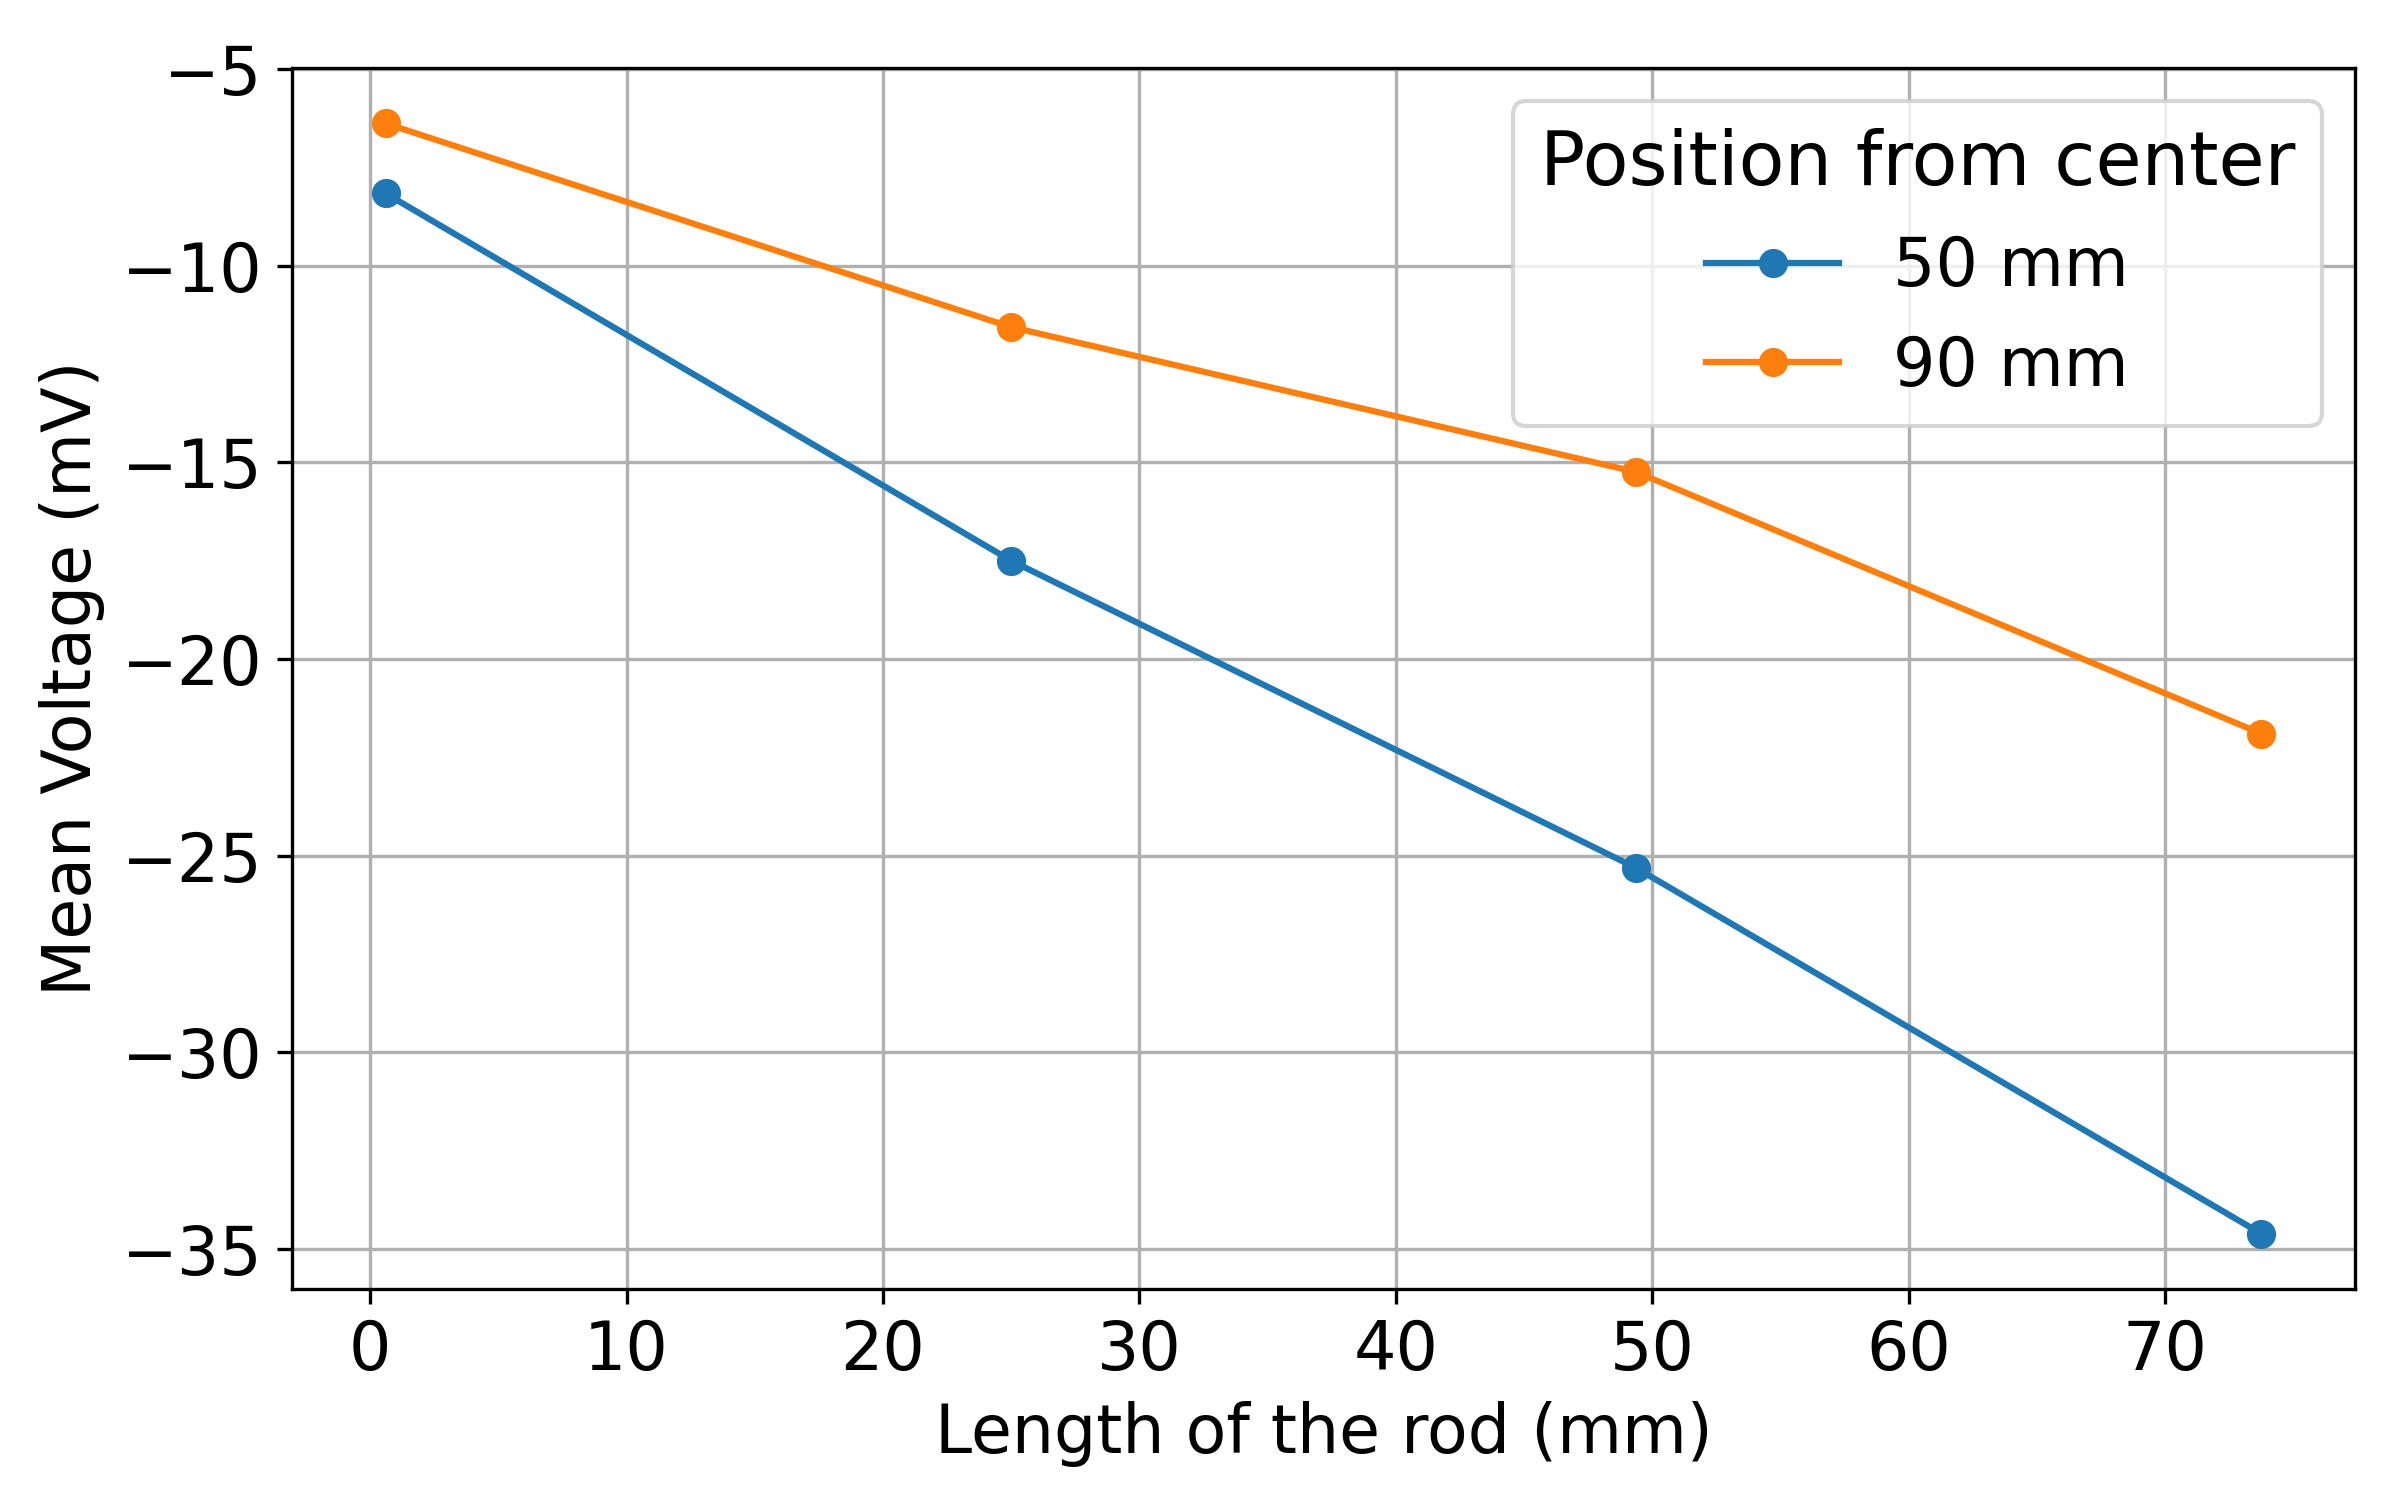
\includegraphics[width=0.85\textwidth]{Assets/1stTrials_50_90.png}
	\caption[Effect of sensor position on mean sensor voltage response]{Mean voltage response of the sensor as a function of length ($L$) for different distances  ($r$) from the center (50--90 mm). 
		At larger lengths (farther from the strain gauges) an increase in signal reading.
		Further from the rotation axis the measurements diverge, showing higher sensitivity near the center (50 mm). }
	\label{fig:posAndHeight}
\end{figure}

Figure \ref{fig:torque_fit} demonstrates the expected inverse relation of force and position along the transfer arm from the rotation axis ($1/r$) in two ways. First Figure \ref{fig:loglogtorque} shows a log-log plot voltage vs position with a fit n value very close to -1. Additionally, a $A/r$ fit (Figure \ref{fig:ABfittorque}) provides the constant $A$, also very close to -1. This signifies, it is a good method to measure torque via the counter force. 

\begin{figure}[hbt!]
	\centering
	
	\subfloat[\label{fig:loglogtorque}]{
		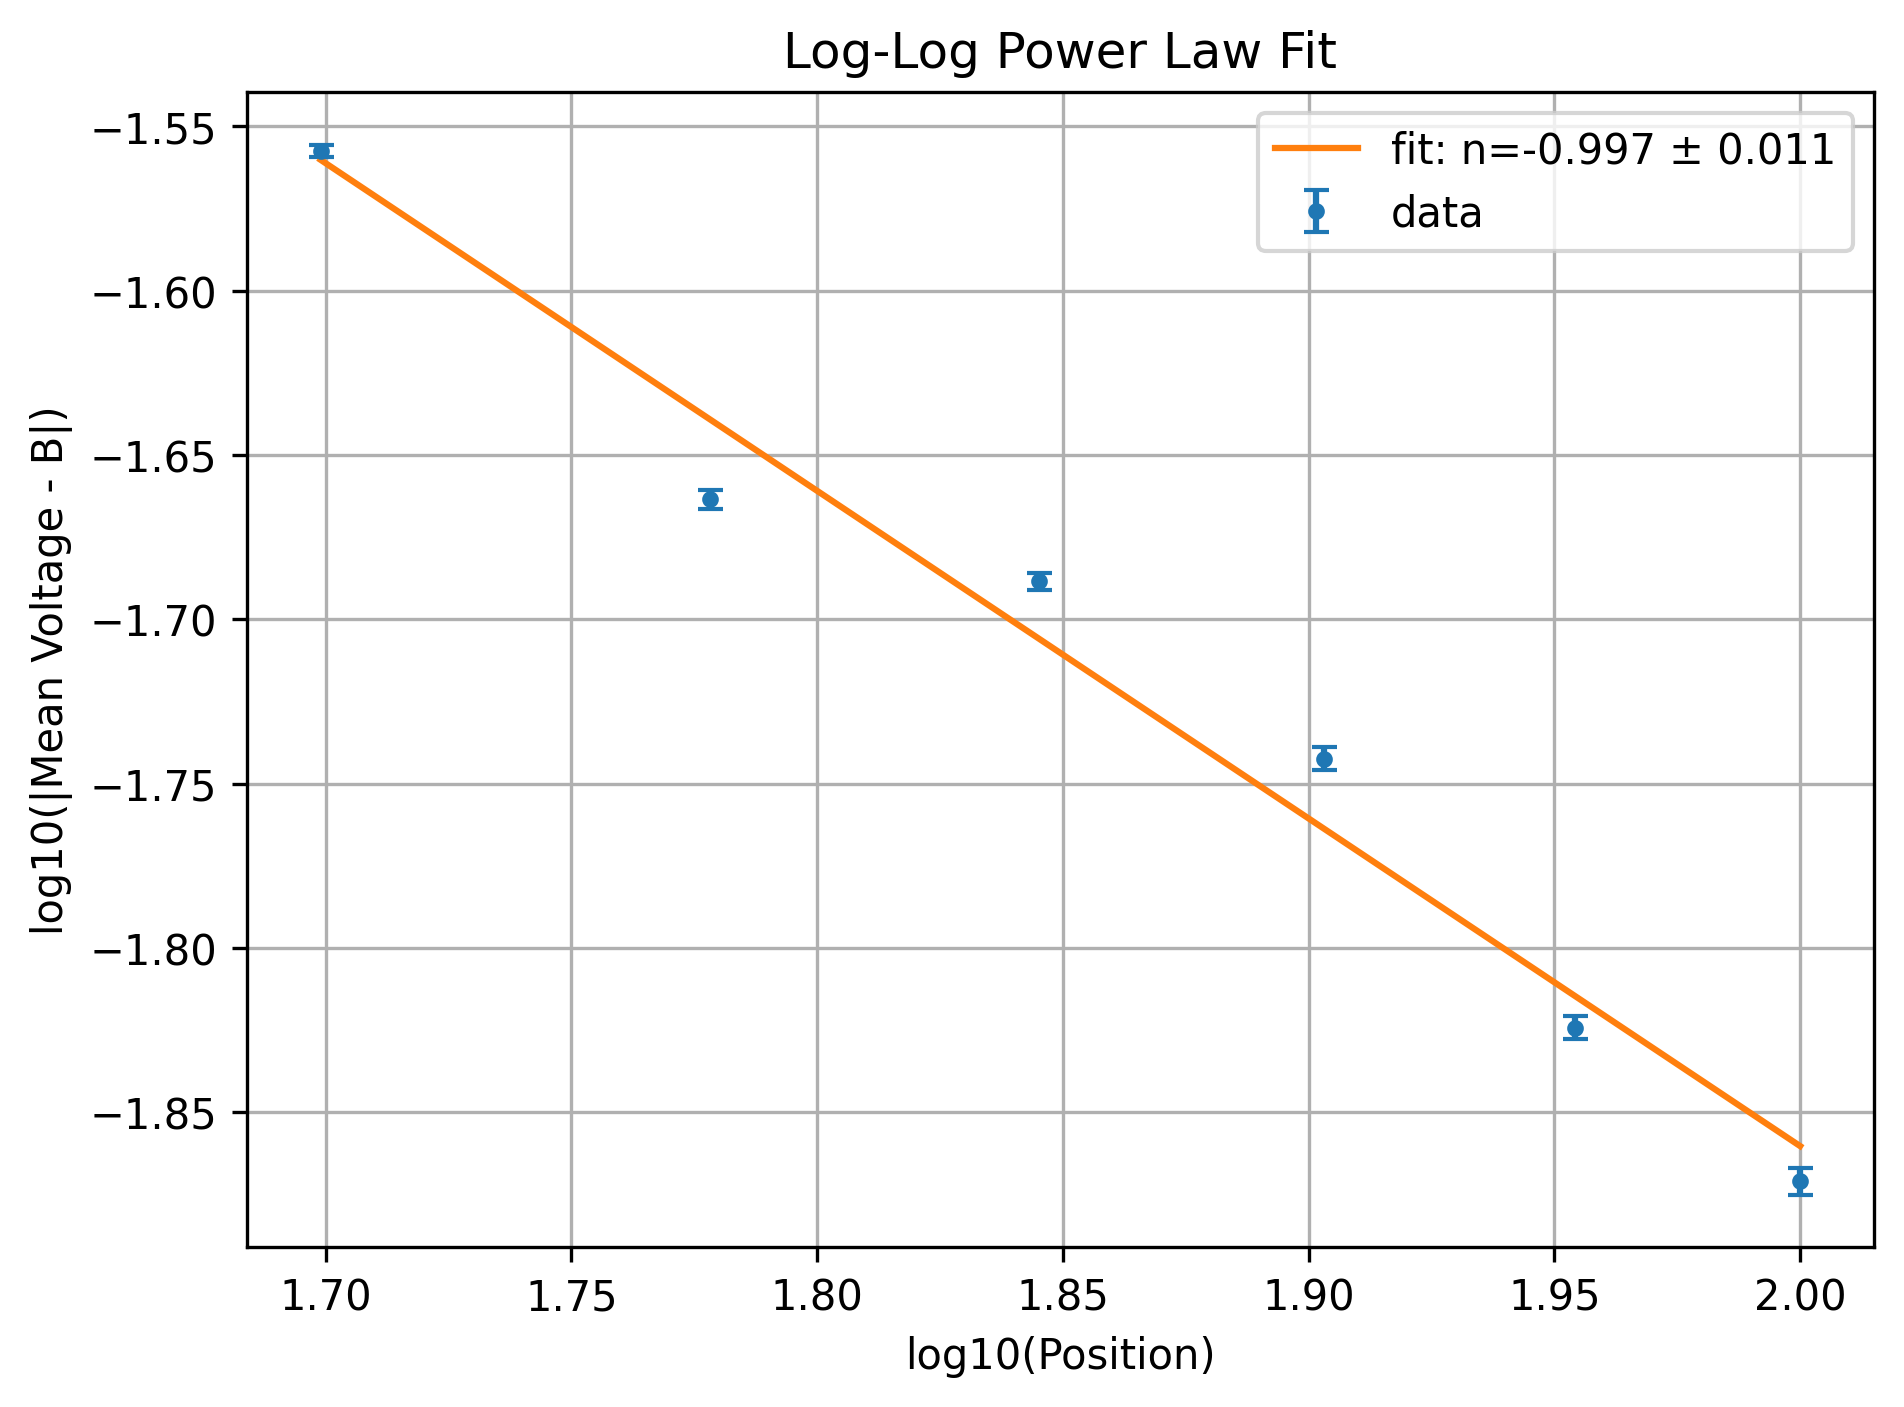
\includegraphics[width=0.85\textwidth]{Assets/powerFitFr.png}
	}
	\hfill
	\subfloat[\label{fig:ABfittorque}]{
		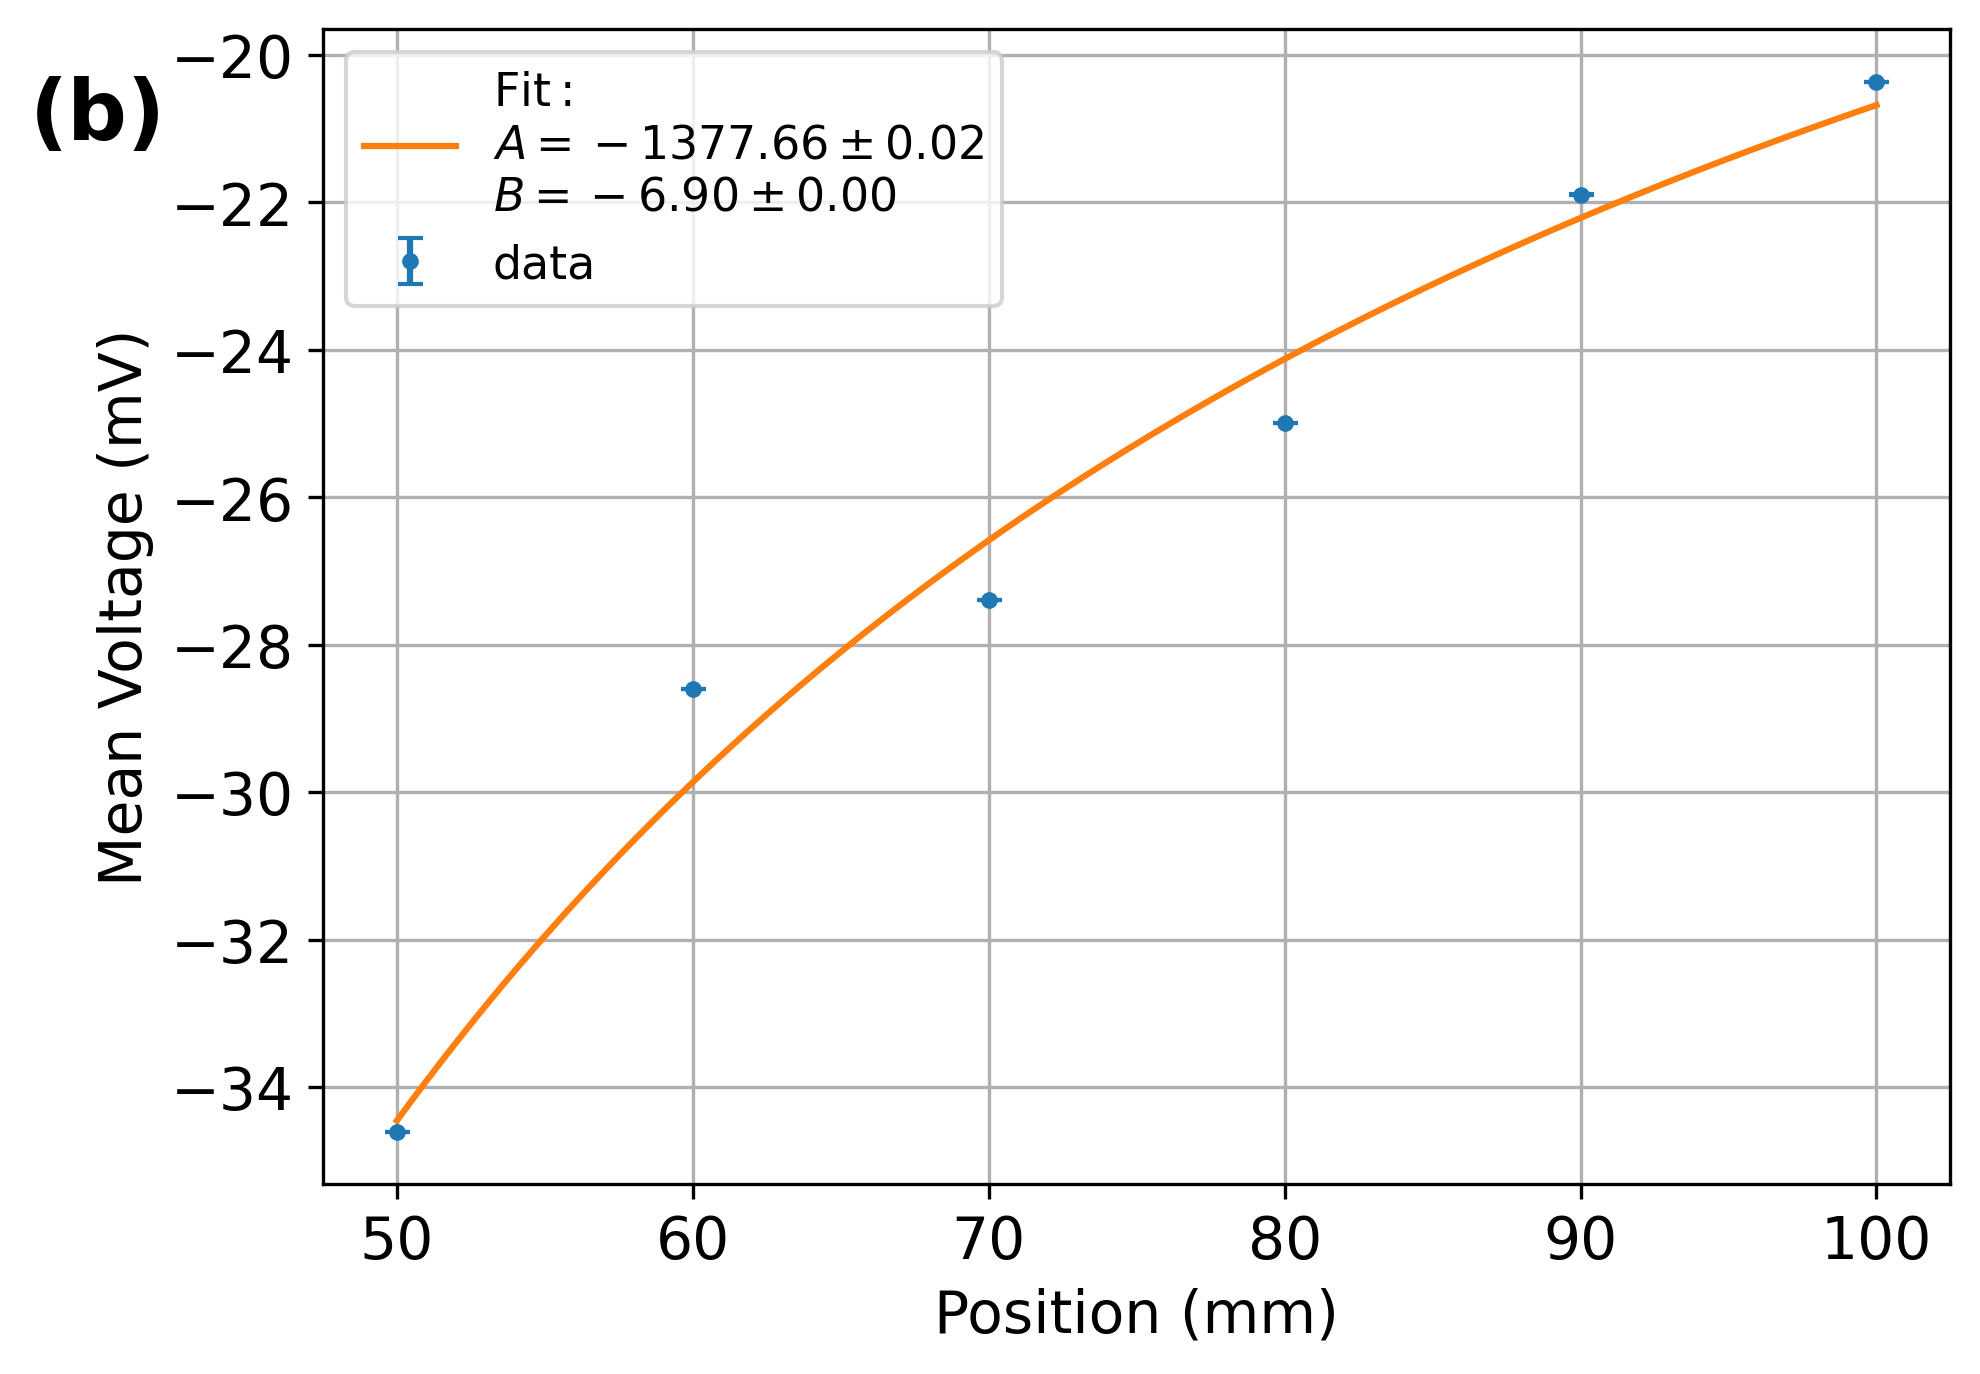
\includegraphics[width=0.85\textwidth]{Assets/inverseRfitFr.png}
	}
	\caption[Expected $1/r$ dependence of torque]{Demonstration of the expected inverse-distance dependence of the force (and thus torque) with respect to the distance $r$ from the rotation axis. Both analyses confirm the $1/r$ dependence characteristic of the torque measurement via counter-force method. (a) Log-log plot of effective measured voltage (proportional to force) versus position $r$, showing a power-law fit with exponent $n = -0.997 \pm 0.011$, very close to the theoretically expected value of $-1$. (b) Direct fit of the form $F(r) = A/r + B$, yielding $A = -1.378 \pm 0.015$ (very close to $-1$ in normalized units) and a negligible offset $B = -0.0069 \pm 0.0002$.}
	\label{fig:torque_fit}
\end{figure}

Once the sensor and circuit were calibrated and the best position for measurement in the torque fixture are affixed, we moved on to the in laboratory measurements of torque in Section \ref{sec:sensorCal}. 

\FloatBarrier

\subsection{Torque from Lab scale magnet}

As described in section \ref{sec:InLab_Torque}, torque measurements were performed under three different experimental configurations. When a small uniform magnetic field was applied using Helmholtz coils, the torque produced by the short (2 cm) magnetic dowel remained at or below the detection limit of the measurement system. For that reason, only the longer rod yielded reliable results. Figure \ref{fig:torque_longerRod} shows the maximum torque (N m) against the magnetic flux experimental data (in blue) exhibiting a clear parabolic dependence on $  B  $.

\begin{figure}[htb!]
	\label{fig:torque_longerRod}
	\centering
	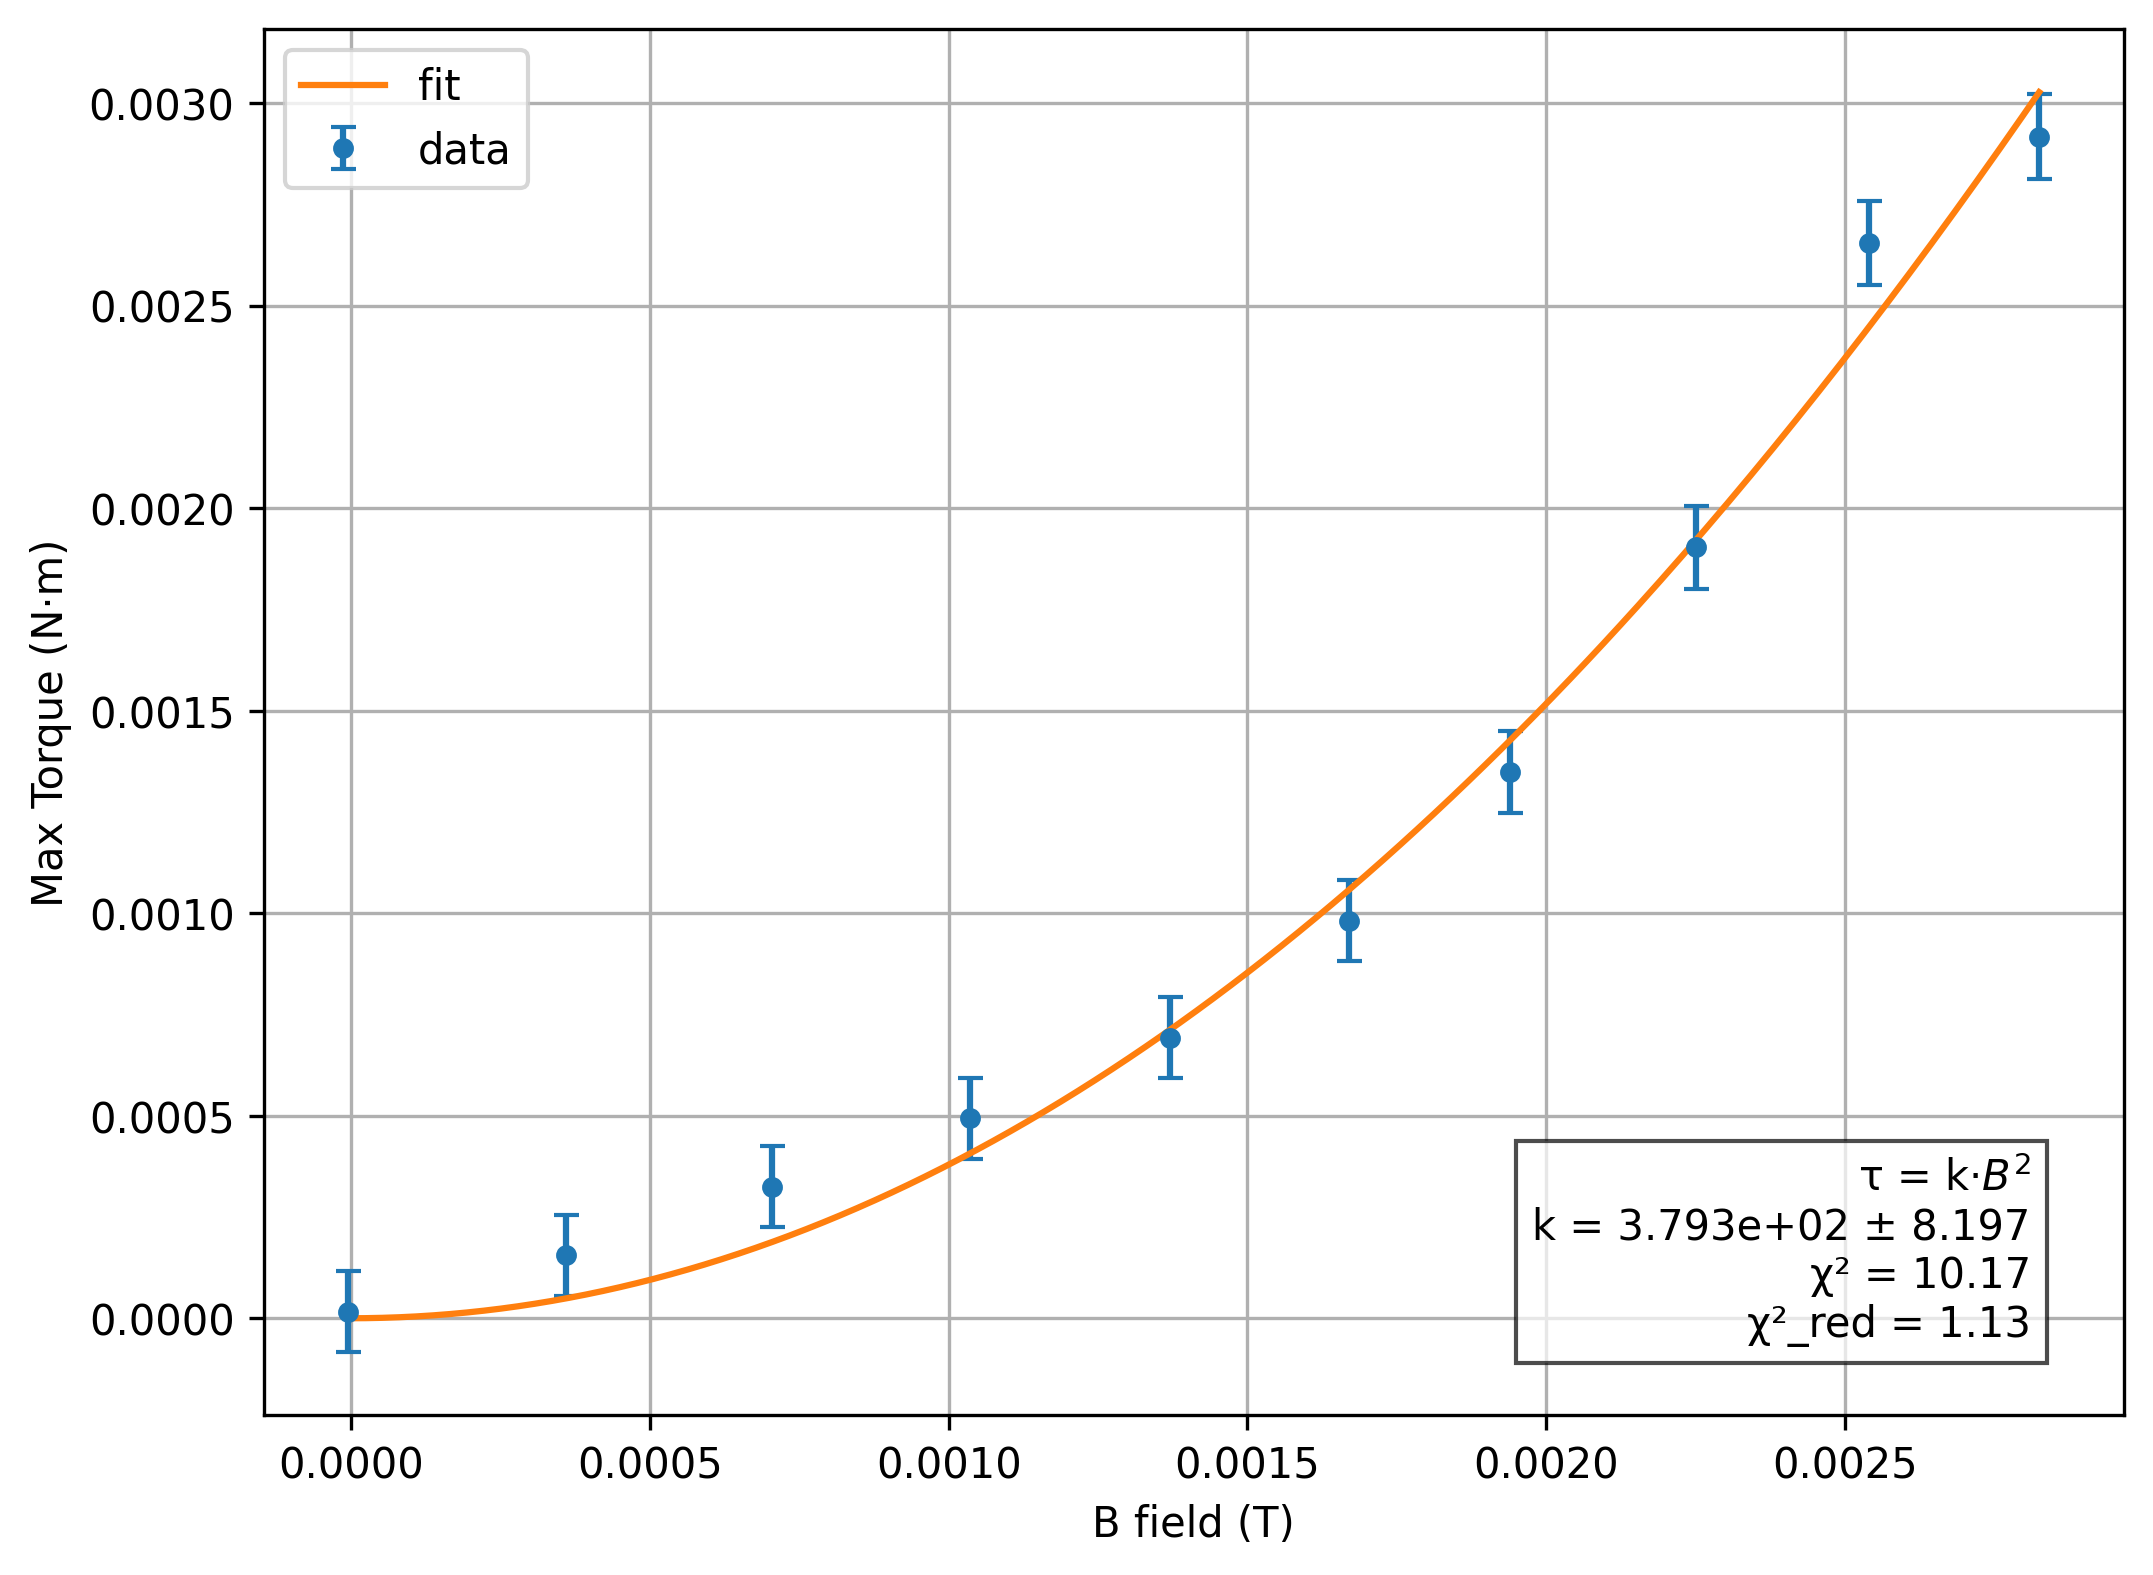
\includegraphics[width=0.85\textwidth]{Assets/example_plot.png}
	\caption[Torque vs. magnetic field strength for the longer rod under Helmholtz coils]{Maximum measured torque in Nm as a function of applied magnetic flux density in B for the longer rod under a Helmholtz coil configuration.}
\end{figure}

From the fit parameters, $k = 3.87 \pm 44.5$, $b = -5.56\times10^{-2}$ and $V_0 = 8.45 \times 10 ^{-5}$. The dominant quadratic term ($  k B^2  $) is in excellent agreement with the theoretical expectation for the torque on a magnetic dipole in a uniform field, where $  \tau \propto B^2  $. The linear coefficient $  b  $ is very small and statistically consistent with zero within uncertainty, while the offset $  V_0  $ is negligible, confirming the absence of significant systematic bias in the measurement.


A second set of measurements was performed on the shorter (2,cm) magnetic dowel using significantly stronger magnetic fields generated by four neodymium magnets. Figure \ref{fig:torque_shorterRod} shows a parabolic relationship, however the values on torque are smaller for higher magnetic fields 

\begin{figure}[htb!]
	\label{fig:torque_shorterRod}
	\centering
	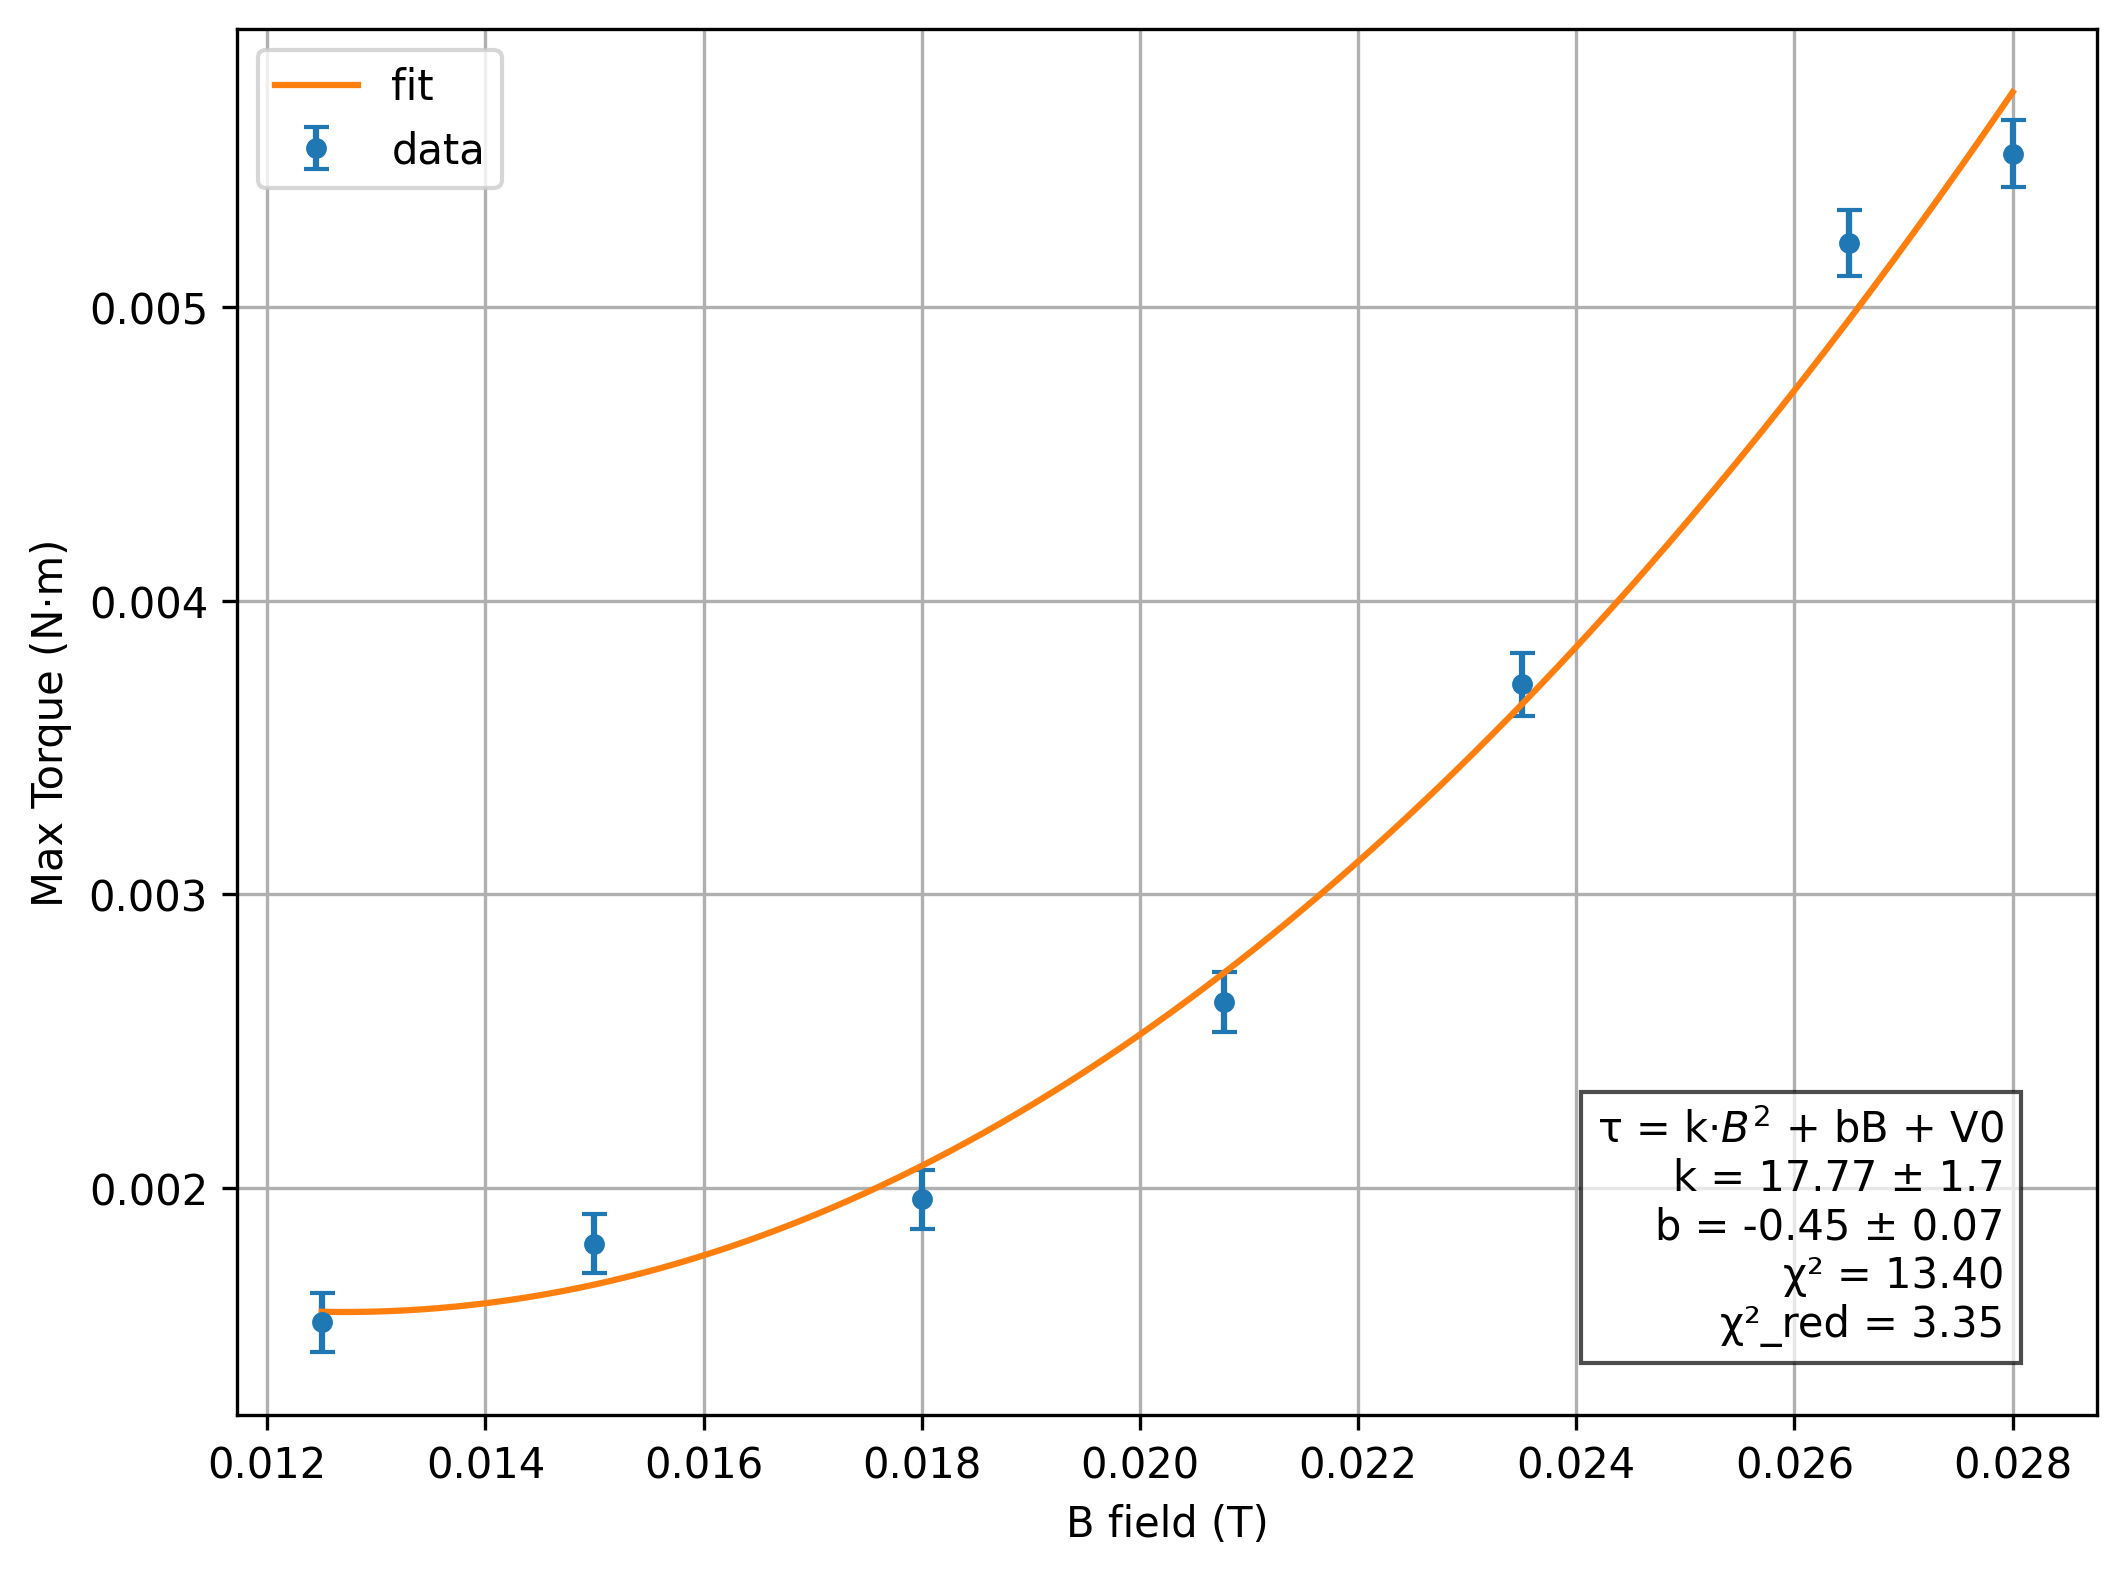
\includegraphics[width=0.85\textwidth]{Assets/example_plotS.png}
	\caption[Torque dependence on magnetic field strength for 2 cm rod under neodymium magnet fields]{Maximum torque in Nm as a function of applied magnetic flux density in T for the shorter (2cm) magnetic rod under stronger uniform fields (Neodymium magnets). Blue points is the experimental measurements while orange curve represents a quadratic fit}
\end{figure}

This time the fit yielded, 

\subsection{Torque from 3T Siemens Magnetom\textsuperscript{\texttrademark} \gls{mri} scanner}

Once in a clinical environment, both the circuit and the \gls{mri}-safe torque measuring fixture were functioning properly and circuit calibration was appropriate for clinical measurements. 

After a single session in the \gls{mri} room no torque was perceived. Neither test material shown any perceptible or measurable torque inside the scanner. 

Despite these efforts, no measurable torque-induced deflection or angular shift was detected on the sensor readout for either material.

The 316L stainless steel rods were found to be too short or too thin to generate detectable torque under the prevailing fringe-field conditions, indicating that longer segments, greater mass, or increased ferromagnetic contribution would be necessary to elicit observable effects in future iterations. Titanium rods likewise produced no response, aligning with expectations for its weakly paramagnetic properties in clinical \gls{mri} environments.

In total, several positioning attempts were made at central and progressively closer locations to the bore, but no quantifiable torque data could be obtained. The protocol ultimately failed to yield reliable torque measurements due to insufficient induced effect on the tested sample configurations. These observations highlight the need for more substantial material samples in subsequent testing to amplify any potential torque for characterization. 

\FloatBarrier
%from lab to clinic expected torque

\section{Key Findings}

